% Options for packages loaded elsewhere
\PassOptionsToPackage{unicode}{hyperref}
\PassOptionsToPackage{hyphens}{url}
\PassOptionsToPackage{dvipsnames,svgnames*,x11names*}{xcolor}
%
\documentclass[]{article}
\usepackage{lmodern}
\usepackage{amssymb,amsmath}
\usepackage{ifxetex,ifluatex}
\ifnum 0\ifxetex 1\fi\ifluatex 1\fi=0 % if pdftex
  \usepackage[T1]{fontenc}
  \usepackage[utf8]{inputenc}
  \usepackage{textcomp} % provide euro and other symbols
\else % if luatex or xetex
  \usepackage{unicode-math}
  \defaultfontfeatures{Scale=MatchLowercase}
  \defaultfontfeatures[\rmfamily]{Ligatures=TeX,Scale=1}
\fi
% Use upquote if available, for straight quotes in verbatim environments
\IfFileExists{upquote.sty}{\usepackage{upquote}}{}
\IfFileExists{microtype.sty}{% use microtype if available
  \usepackage[]{microtype}
  \UseMicrotypeSet[protrusion]{basicmath} % disable protrusion for tt fonts
}{}
\makeatletter
\@ifundefined{KOMAClassName}{% if non-KOMA class
  \IfFileExists{parskip.sty}{%
    \usepackage{parskip}
  }{% else
    \setlength{\parindent}{0pt}
    \setlength{\parskip}{6pt plus 2pt minus 1pt}}
}{% if KOMA class
  \KOMAoptions{parskip=half}}
\makeatother
\usepackage{xcolor}\pagecolor[RGB]{28,30,38} \color[RGB]{213,216,218}
\IfFileExists{xurl.sty}{\usepackage{xurl}}{} % add URL line breaks if available
\IfFileExists{bookmark.sty}{\usepackage{bookmark}}{\usepackage{hyperref}}
\hypersetup{
  pdftitle={Fourier Analysis and the Theory of Distributions},
  pdfauthor={Kexing Ying},
  colorlinks=true,
  linkcolor=Maroon,
  filecolor=Maroon,
  citecolor=Blue,
  urlcolor=red,
  pdfcreator={LaTeX via pandoc}}
\urlstyle{same} % disable monospaced font for URLs
\usepackage[margin = 1.5in]{geometry}
\usepackage{graphicx}
\makeatletter
\def\maxwidth{\ifdim\Gin@nat@width>\linewidth\linewidth\else\Gin@nat@width\fi}
\def\maxheight{\ifdim\Gin@nat@height>\textheight\textheight\else\Gin@nat@height\fi}
\makeatother
% Scale images if necessary, so that they will not overflow the page
% margins by default, and it is still possible to overwrite the defaults
% using explicit options in \includegraphics[width, height, ...]{}
\setkeys{Gin}{width=\maxwidth,height=\maxheight,keepaspectratio}
% Set default figure placement to htbp
\makeatletter
\def\fps@figure{htbp}
\makeatother
\setlength{\emergencystretch}{3em} % prevent overfull lines
\providecommand{\tightlist}{%
  \setlength{\itemsep}{0pt}\setlength{\parskip}{0pt}}
\setcounter{secnumdepth}{5}
\usepackage{tikz}
\usepackage{physics}
\usepackage{amsthm}
\usepackage{mathtools}
\usepackage{esint}
\usepackage[ruled,vlined]{algorithm2e}

\usepackage{pgfplots}
\pgfplotsset{width=8cm,compat=1.9}
\usetikzlibrary{external} % cache the plot
\tikzexternalize[prefix=pgfplots/]

\theoremstyle{definition}
\newtheorem{theorem}{Theorem}
\newtheorem{definition*}{Definition}
\newtheorem{prop}{Proposition}
\newtheorem{corollary}{Corollary}[theorem]
\newtheorem*{remark}{Remark}
\theoremstyle{definition}
\newtheorem{definition}{Definition}[section]
\newtheorem{lemma}{Lemma}[section]
\newtheorem{proposition}{Proposition}[section]
\newtheorem{example}{Example}[section]
\newcommand{\diag}{\mathop{\mathrm{diag}}}
\newcommand{\Arg}{\mathop{\mathrm{Arg}}}
\newcommand{\hess}{\mathop{\mathrm{Hess}}}

% the redefinition for the missing \setminus must be delayed
\AtBeginDocument{\renewcommand{\setminus}{\mathbin{\backslash}}}

\title{Fourier Analysis and the Theory of Distributions}
\author{Kexing Ying}

\begin{document}
\maketitle

{
\hypersetup{linkcolor=}
\setcounter{tocdepth}{2}
\tableofcontents
}
\newpage

\section{Orthonormal System}

We will in this section recall some results about orthonormal systems in Euclidean 
spaces\footnote{In this course, we shall call real inner product spaces Euclidean 
spaces.} and generalize them to complex spaces. 

\subsection{Euclidean Space}

\begin{definition}
  A system of nonzero vectors \(\{X_\alpha\} \subseteq R\) where \(R\) is an 
  Euclidean space is called orthogonal if \(\langle X_\alpha, X_\beta\rangle = 0\)
  for all \(\alpha \neq \beta\). 

  In addition, if for all \(\alpha\), \(\langle X_\alpha, X_\alpha\rangle = 1\), 
  we say the system is orthonormal.
\end{definition}

Clearly, given an orthogonal system \(\{X_\alpha\}\), we may normalize the vector 
such that \(\{X_\alpha / \|X_\alpha\|\}\) is an orthonormal system. Furthermore, 
recall that a system of orthogonal vectors is linearly independent.

\begin{definition}
  A complete (i.e. the smallest closed subspace containing the system is \(R\)) 
  orthogonal system \(\{X_\alpha\} \subseteq R\) is said to 
  be an orthogonal basis of \(R\). 
\end{definition}

Some important spaces we shall study in this course include \(\mathbb{R}^2\) 
(equipped with the Euclidean norm), \(l_2\), \(\mathcal{C}([-\pi , \pi])\) 
(the space of continuous functions on \([-\pi, \pi]\) equipped with the \(L_2\) norm). 

\begin{proposition}
  Let \(R\) be a separable Euclidean space. Then any orthogonal system in \(R\) 
  is countable. 
\end{proposition}
\begin{proof}
  By normalizing, we may assume the system \(\{X_\alpha\}\) is orthonormal. Then, 
  for \(\alpha \neq \beta\),
  \[\|X_\alpha - X_\beta\|^2 = \|X_\alpha\|^2 - 2\langle X_\alpha, X_\beta\rangle + 
  \|X_\beta\|^2 = \|X_\alpha\|^2 + \|X_\beta\|^2 = 2.\]
  Then, \(B_{1 / 2}(X_\alpha) \cap B_{1 / 2}(X_\beta) = \varnothing\) for all 
  \(\alpha \neq \beta\). Thus, if the system is not countable, we have found 
  a uncountable number of disjoint open balls, contradicting the separability of 
  \(R\).
\end{proof}

\begin{proposition}
  Let \(f_1, f_2, \cdots\) be a linearly independent system in a Euclidean space 
  \(R\). Then, there exists an orthonormal system \(\phi_1, \phi_2, \cdots\) such 
  that 
  \[\phi_n = a_{n_1} f_1 + \cdots + a_{n_n} f_n\]
  and 
  \[f_n = b_{n_1}\phi_1 + \cdots + b_{n_n} \phi_n\]
  for some \(a_{n_k}, b_{n_k} \in \mathbb{R}\) and \(a_{n_n}, b_{n_n} \neq 0\).
  Furthermore, the system \(\phi_1, \phi_2, \cdots\) is uniquely determined up 
  to a multiplication by \(\pm 1\).
\end{proposition}
\begin{proof}
  Use Gram-Schmidt. 
\end{proof}

\begin{corollary}
  A separable Euclidean space \(R\) possesses an orthonormal basis.
\end{corollary}
\begin{proof}
  Simply obtain the orthonormal system corresponding to the countable dense 
  system of \(R\). The resulting system is complete since the two systems have the 
  same linear closure.
\end{proof}

\begin{definition}[Fourier Coefficients]
  Let \(\phi_1, \phi_2, \cdots\) be an orthonormal system in \(R\) and let \(f \in R\). 
  Consider the sequence \(c_k = \langle f, \phi_k \rangle\) for all \(k = 1, 2, \cdots\). 
  Then \(c_k\) are called the coordinates or Fourier coefficients of \(f\) with respect 
  to the system \(\{\phi_k\}\) and \(\sum_{k = 1}^\infty c_k \phi_k\) is 
  called the Fourier series of \(f\).
  
  Note that this series in the definition is a formal series as we do not yet 
  know whether or not the series converges.
\end{definition}

In the finite case, it is not difficult to see that the sequence 
\(\alpha_k\) for \(k = 1, \cdots, n\) which minimizes \(\|f - S_n^{(\alpha)}\|\) 
where \(S_n^{(\alpha)} := \sum_{k = 1}^n \alpha_k \phi_k\) is the Fourier coefficients. 
Indeed, we have 
\[\begin{split}
  \|f - S_n^{(\alpha)}\|^2 & = \langle f, f \rangle - 2 \langle f, S_n^{(\alpha)} \rangle +
    \langle S_n^{(\alpha)}, S_n^{(\alpha)} \rangle\\
    & = \|f\|^2 - 2 \sum \alpha_k c_k + \sum \alpha_k^2\\
    & = \|f\|^2 - \sum c_k^2 + \sum (\alpha_k - c_k)^2.
\end{split}\]
Hence, \(\|f - S_n^{(\alpha)}\|\) is minimized when \(\alpha_k = c_k\) for all 
\(k = 1, \cdots, n\). With this in mind, choosing \(\alpha\) to be the Fourier 
coefficients, we have 
\[\|f - S_n^{(c)}\| = \|f\|^2 - \sum_{k = 1}^n c_k^2.\]
Geometrically, \(f - S_n^{(\alpha)}\) is orthogonal to the subspace generated by 
\(\phi_1, \cdots, \phi_n\) if and only if \(\alpha = c\).

Furthermore, by noting \(0 \le \|f - S_n^{(c)}\| = \|f\|^2 - \sum_{k = 1}^n c_k^2\), 
we have 
\[\sum_{k = 1}^n c_k^2 \le \|f\|^2 < \infty,\]
and hence, taking \(n \to \infty\), we have \(\sum_{k = 1}^\infty c_k^2\) exists 
and is bounded above by \(\|f\|^2\). This inequality is known as the Bessel inequality.

\begin{definition}[Closed Orthonormal System]
  The orthonormal system \(\{\phi_k\}\) is closed if for any \(f \in R\), we have 
  \[\sum_{k = 1}^\infty c_k^2 = \|f\|^2.\]
  This property is called the Parseval equality.
\end{definition}

Again, by observing \(\|f - S_n^{(c)}\| = \|f\|^2 - \sum_{k = 1}^n c_k^2\),
the system is closed if and only if for any \(f\), the partial sums of the 
Fourier series converge to \(f\), i.e. \(f = \sum_{k = 1}^\infty c_k \phi_k\).

\begin{proposition}
  In a separable Euclidean space \(R\), an orthonormal system is complete 
  if and only if it is closed.
\end{proposition}
\begin{proof}
  Suppose first that \(\{\phi_k\}\) is closed. Then, for all \(f \in R\), 
  \(f = \sum_{k = 1}^\infty c_k \phi_k\). Thus, the finite linear combinations of 
  \(\{\phi_k\}\) is dense in \(R\) and thus, \(\{\phi_k\}\) is complete.

  On the other hand, suppose that \(\{\phi_k\}\) is complete (it is countable 
  as \(R\) is separable), for any \(f \in R\), there exists some \(\alpha^k\) 
  such that \(\|f - S^{(\alpha^k)}_\infty\| \to 0\). As we have seen, for any partial 
  sum \(S^{(\alpha^k)}_n\), we have \(\|f - S^{(c)}_n\| \le \|f - S^{(\alpha^k)}_n\|\) 
  and so, 
  \[\|f - S^{(c)}_\infty\| \le \|f - S^{(\alpha^k)}_\infty\| \to 0\]
  implying \(\|f - S^{(c)}_\infty\| = 0\) and the system is closed.
\end{proof}


\begin{proposition}
  Given \(f, g \in R\) and a closed orthonormal system \(\{\phi_k\}\), 
  \[\langle f, g \rangle = \sum_{k = 1}^\infty c_k d_k\]
  where \((c_k), (d_k)\) are the Fourier coefficients of \(f\) and \(g\) with respect 
  to \(\{\phi_k\}\) respectively.
\end{proposition}
\begin{proof}
  We have, by Parseval's identity, \(\|f\|^2 = \sum c_k^2\), \(\|g\|^2 = \sum d_k^2\) 
  and \(\|f + g\|^2 = \sum (c_k + d_k)^2 = \sum c_k^2 + 2 \sum c_k d_k + \sum d_k^2\),
  we have 
  \[\sum c_k^2 + 2 \sum c_k d_k + \sum d_k^2 = \|f + g\|^2 = \|f\|^2 + 2\langle f, g\rangle + \|g\|^2.\]
  Thus, cancelling using \(\|f\|^2 = \sum c_k^2\) and \(\|g\|^2 = \sum d_k^2\), we have 
  \(\langle f, g \rangle = \sum_{k = 1}^\infty c_k d_k\) as required.
\end{proof}

In the case the system is only orthogonal but not necessary orthonormal, we may 
normalize the Fourier coefficients, i.e. given an orthogonal system \(\{\phi_k\}\), 
we have \(\{\phi / \|\phi_k\|\}\) is an orthonormal system, and so, we define
\[c_k = \left\langle f, \frac{\phi_k}{\|\phi_k\|} \right\rangle = \frac{1}{\|\phi_k\|} \langle f, \phi_k \rangle.\]
Similarly, the Fourier series of \(f\) is becomes 
\[\sum_{k = 1}^\infty c_k \frac{\phi_k}{\|\phi_k\|} = \sum \frac{\langle f, \phi_k\rangle}{\|\phi_k\|^2} \phi_k.\]
Substituting this definition of the Fourier coefficients into the Bessel inequality,
we obtain 
\[\sum_{k = 1}^\infty \frac{\langle f, \phi_k\rangle^2}{\|\phi_k\|^2} \le \|f\|^2,\]
for any orthogonal system \(\{\phi_k\}\).

\begin{theorem}[Riesz]
  Let \(\{\phi_k\}\) be a orthonormal system in a complete Euclidean space \(R\) 
  (i.e. a real Hilbert space) and let \(c \in \ell_2\) 
  (i.e. \(\sum_{k = 1}^\infty c_k^2 < \infty\)). Then, 
  there exists some \(f \in R\) such that \(c_k = \langle f, \phi_k \rangle\) and 
  Parseval's identity holds, i.e.
  \[\sum_{k = 1}^\infty c_k^2 = \|f\|^2.\]
\end{theorem}
\begin{proof}
  Let \(f_n := \sum_{k = 1}^n c_k \phi_k\). Then, by definition, we have 
  \(c_k = \langle f_n, \phi_k \rangle\) for all \(k = 1, \cdots, n\). Then, 
  for all \(p \ge 1\), we have
  \[\|f_{n + p} - f_n\|^2 = \|c_{n + 1} \phi_{n + 1} + \cdots + c_{n + p} \phi_{n + p}\|^2 
    = \sum_{k = n + 1}^{n + p} c_k^2.\]
  Now, as \(\sum c_k^2 < \infty\), we have \(\{f_n\}\) is Cauchy, and thus, as 
  \(R\) is complete, there exists some \(f \in R\) such that \(f_n \to f\). 
  Thus, by noting, 
  \[\langle f, \phi_k \rangle = \langle f_n \phi_k\rangle + \langle f - f_n, \phi_k\rangle
    = c_k + \langle f - f_n, \phi_k\rangle,\]
  where \(\langle f - f_n, \phi_k\rangle \to 0\) as \(n \to \infty\) since 
  \(|\langle f - f_n, \phi_k\rangle| \le \|f - f_n\| \|\phi_k\|\) by the 
  Cauchy-Schwarz inequality, we have \(c_k = \langle f, \phi_k\rangle\).

  Finally, Parseval's identity, follows as \(\|\cdot\|^2\) is continuous in a 
  normed space.
\end{proof}

Let us recall the following result from functional analysis.

\begin{proposition}
  Any separable Hilbert space is isomorphic to \(\ell_2\) (thus, any two separable 
  Hilbert spaces are isomorphic). 
\end{proposition}
\begin{proof}
  Let \(H\) be a separable Hilbert space and choose \(\{\phi_k\}\) a complete 
  orthonormal system (which exists as \(H\) is separable). Then, for any \(f \in H\), 
  we map \(f\) to the sequence corresponding to its Fourier coefficients, i.e.
  \[\psi : f \mapsto (c_1, c_2, \cdots)\]
  which is well-defined by Bessel's inequality. On the other hand, by Riesz's 
  theorem, for any \(x \in \ell_2\), \(\sum x_k^2 < \infty\) and so, there 
  exists a unique \(f \in H\),  such that \(\psi(f) = x\). Thus, as \(\psi\) is 
  clearly linear (as the inner products are linear with respect to the left 
  component), we have the isomorphism between \(H\) and \(\ell_2\).
\end{proof}

\subsection{Complex Inner Product Space}

We will in the course take the complex inner product to be anti-linear in the 
second component. As promised earlier, most definitions can be generalized 
from the real case to the complex directly.

\begin{definition}[Fourier Coefficients]
  Let \(R\) be a complex inner product space. Then, for an orthonormal system 
  \((\phi_n)\) and \(f \in R\), we define its Fourier coefficients to be 
  \(c_k := \langle f, \phi_k\rangle\) for all \(k = 1, \cdots, n\). Similarly,
  we define the Fourier series of \(f\) to be the formal series 
  \(\sum_{k = 1}^\infty c_k \phi_k\).
\end{definition}

Going through the same argument as the real case, we obtain the complex version 
of Bessel's inequality.

\begin{proposition}[Bessel's Inequality]
  Given an orthonormal system \((\phi_n)\) and \(f \in R\), we have 
  \[\sum_{k = 1}^\infty |c_k|^2 \le \|f\|^2.\]
\end{proposition}

Going through all proved theorems for real spaces, we find they also hold for 
complex spaces (with trivial modifications).

\newpage
\section{Fourier Series}

\subsection{Trigonometric Series}

We will consider the space \(L_2[-\pi, \pi]\) (the space of square-integrable functions 
from \([-\pi, \pi]\) quotiented by the a.e.-equal equivalence relation equipped with 
the inner product \(\langle f, g\rangle := \int_{[-\pi, \pi]} fg \dd\lambda\)), and the 
trigonometric system 
\[\{\mathbf{1}, \cos(n x), \sin(n x) \mid n = 1, 2, \cdots\}.\]
It is not difficult to see that this system is orthogonal, but in fact, it is 
also complete. Indeed, completeness follows by the Weierstrass approximation theorem 
for trigonometric polynomials (we will discuss this later / recall the Stone-Weierstrass 
theorem and observe that the trigonometric system seperates points).

Nonetheless, this system is not orthonormal, and thus, we normalise the system 
such that the system becomes 
\[\left\{\frac{1}{\sqrt{2\pi}}\mathbf{1}, \frac{1}{\sqrt{\pi}}\cos(n x), \frac{1}{\sqrt{\pi}}\sin(n x) \mid n = 1, 2, \cdots\right\}.\]
Hence, the Fourier series of an element \(f \in L_2[-\pi, \pi]\) becomes the 
famous formula
\[\frac{a_0}{2} + \sum_{k = 1}^\infty (a_k \cos kx + b_k \sin k x),\]
where 
\[a_k := \frac{1}{\pi}\int_{[-\pi, \pi]} f(x) \cos(k x) \lambda(\dd x),
  b_k := \frac{1}{\pi}\int_{[-\pi, \pi]} f(x) \sin(k x) \lambda(\dd x).\]
By recalling the above theory, the \(n\)-th partial sum of this series provides the best 
(in \(L_2\) metric) approximation of \(f\) among all trigonometric polynomials 
of degree \(n\). Hence, as the trigonometric system is complete, Parseval's 
identity holds, and so, 
\[\|f - S_n\|_2 \to 0, \text{ as } n \to \infty.\]
By observing that \(e^{ix} = \cos x + i\sin x\), we may rewrite the Fourier series 
can be written in the complex form. In particular, \(L_2[-\pi, \pi]\) has the 
orthogonal system \(\{e^{inx} \mid n \in \mathbb{Z}\}\) and the Fourier series 
of \(f \in L_2[-\pi, \pi]\) is given by 
\[\sum_{n = -\infty}^\infty c_n e^{inx}, \text{ where }
  c_n = \frac{1}{2\pi} \int_{[-\pi, \pi]} f(x)e^{-inx}\lambda(\dd x).\]
\begin{itemize}
  \item Since a function on \([-\pi, \pi]\) can be extended to \(\mathbb{R}\) by periodicity, 
    we can, instead of functions on \([-\pi, \pi]\) consider periodic functions with 
    period \(2\pi\) on \(\mathbb{R}\).
  \item Since \(\cos nx, \sin nx\) are bounded functions, the integrals defining 
    the trigonometric Fourier coefficients exists for any function in \(L_1[-\pi, \pi]\), 
    i.e. if \(f \in L_1[-\pi, \pi]\), then 
    \[\int f \cos(nx), \int f\sin(nx) < \int |f| < \infty.\]
  \item \(L_2[-\pi, \pi] \subseteq L_1[-\pi, \pi]\) by Hölder's inequality and thus,
    with the above remark in mind, the definition of Fourier series is also well-defined 
    for any integrable functions (though convergence is much opaque in this case).
\end{itemize}
While the Fourier series of \(f\) converges to \(f\) in \(L_2\) though it 
is not clear that the Fourier series converges point-wise to \(f\) 
(it might be interesting to recall that convergence in \(L_p\) implies convergence 
in measure and the existence of a subsequence which converges almost everywhere).  

Consider the partial sum of the Fourier series of \(f \in L_2[-\pi, \pi]\),
\[\begin{split}
  S_n(x) & = \frac{a_0}{2} + \sum_{k = 1}^n (a_k \cos kx + b_k \sin kx)\\
  & = \frac{1}{\pi}{\int_{[-\pi, \pi]} f(t)}\left(\frac{1}{2} + \sum_{k = 1}^n 
    (\cos kx \cos kt + \sin kx \sin kt)\right)\lambda(\dd t)\\
  & = \frac{1}{\pi}{\int_{[-\pi, \pi]} f(t)}\left(\frac{1}{2} + \sum_{k = 1}^n 
  \cos k(t - x)\right)\lambda(\dd t).
\end{split}\]
By noting the identity
\[\frac{1}{2} + \sum_{k = 1}^n \cos ku = \frac{\sin \frac{2n + 1}{2}u}{2\sin \frac{u}{2}},\]
we obtain 
\[S_n(x) = \frac{1}{\pi}{\int_{[-\pi, \pi]} f(t)} 
  \frac{\sin \frac{2n + 1}{2}(t - x)}{2\sin \frac{t - x}{2}} \lambda(\dd t).\]
Finally, by noting the periodicity of \(f\), by change of variable \(z = t - x\),
we obtain 
\[S_n(x) = \int_{[-\pi, \pi]} f(x + z) D_n(z) \lambda(\dd z), \text{ where }
  D_n(z) := \frac{1}{2\pi} \frac{\sin \frac{2n + 1}{2}z}{\sin \frac{z}{2}}\]
and \(D_n\) is known as the Dirichlet kernel. We remark that the Dirichlet kernel 
\(D_n(z)\) tends to \(\frac{2n + 1}{2\pi}\) as \(z \to 0\) and rapidly osculates 
for large \(n\) though this does not impact our calculation as we are dealing 
with a point which has measure 0. 

\begin{center}
  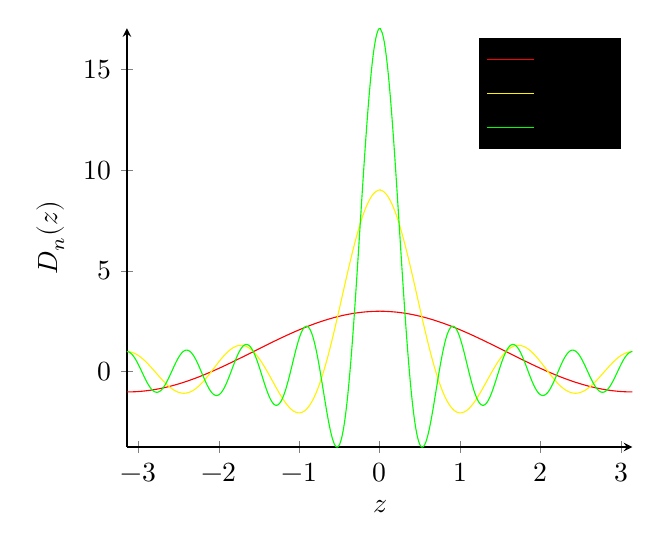
\begin{tikzpicture}
    \begin{axis}[
        legend style={fill=black,draw=white},
        axis lines = left,
        xlabel = \(z\),
        ylabel = {\(D_n(z)\)},
    ]
    %Below the red parabola is defined
    \addplot [
        domain=-pi:pi, 
        samples=500, 
        color=red,
    ]
    {sin(deg((3 / 2) * x)) / sin(deg(x / 2))};
    \addlegendentry{\(n = 1\)}
    %Here the blue parabola is defined
    \addplot [
        domain=-pi:pi, 
        samples=500, 
        color=yellow,
    ]
    {sin(deg((9 / 2) * x)) / sin(deg(x / 2))};    
    \addlegendentry{\(n = 4\)}
    \addplot [
        domain=-pi:pi, 
        samples=500, 
        color=green,
    ]
    {sin(deg((17 / 2) * x)) / sin(deg(x / 2))};    
    \addlegendentry{\(n = 8\)}
  \end{axis}
  \end{tikzpicture}
\end{center}

By observing the graph of the Dirichlet kernel, in some heuristic sense, we note that 
\(D_n(z) \to \delta(z)\) for some function where \(\delta\) is 0 at all points but 
\(z = 0\) while \(\int_{[-\epsilon, \epsilon]} \delta \dd \lambda = 1\) for all 
\(\epsilon > 0\). Such an function cannot exist, however it motivates the second 
part of the course - the theory of distributions.

\subsection{Conditions for Point-wise Convergence}

We observe that \(\|D_n\|_1 = 1\) and so we may write 
\[S_n(x) - f(x) = \int_{[-\pi, \pi]} (f(x + z) - f(x)) D_n(z) \lambda(\dd z).\]
Clearly, \(S_n(x) \to f(x)\) as \(n \to \infty\) if and only if the right hand side
of the above tends to 0. 

\begin{lemma}[Riemann-Lebesgue]
  If \(\phi \in L_1[a, b]\) for some \(a < b\), then both
  \[\int_{[a, b]} \phi(x)\sin (\gamma x) \lambda(\dd x), 
    \int_{[a, b]} \phi(x)\cos (\gamma x) \lambda(\dd x)\]
  tends to 0 as \(\gamma \to \infty\).
\end{lemma}
\begin{proof}
  We will prove the statement for the \(\sin\) case. We observe that if 
  \(\phi\) is continuously differentiable, by integration by parts, we have 
  \[\int_{[a, b]} \phi(x)\sin (\gamma x) \lambda(\dd x) = 
    \left[-\phi(x)\frac{\cos\gamma x}{\gamma}\right]^b_a + 
    \int_{[a, b]} \phi'(x) \frac{\cos \gamma x}{\gamma} \lambda(\dd x),\]
  which tends to 0 as \(\gamma \to \infty\) (we note that \(\phi'\) is continuous 
  on a compact set, and hence bounded above). Now, in the general case, we observe 
  that continuously differentiable functions are everywhere dense in \(L_1[a, b]\), 
  and so, for every \(\epsilon > 0\), there exists some continuously differentiable 
  \(\phi_\epsilon(x)\), such that 
  \[\int_{[a, b]} |\phi - \phi_\epsilon| \dd \lambda = \|\phi - \phi_\epsilon\|_1 < \frac{\epsilon}{2}.\]
  Hence, 
  \[\begin{split}
    \left|\int_{[a, b]} \phi(x) \sin(\gamma x) \lambda(\dd x)\right| 
    & \le \left|\int_{[a, b]} (\phi(x) - \phi_\epsilon(x)) \sin(\gamma x) \lambda(\dd x)\right| 
      + \left| \int_{[a, b]} \phi_\epsilon(x) \sin(\gamma x) \lambda(\dd x)\right|\\
    & \le \|\phi - \phi_\epsilon\|_1 + \left| \int_{[a, b]} \phi_\epsilon(x) \sin(\gamma x) \lambda(\dd x)\right|\\
    & < \frac{\epsilon}{2} + 
    \left| \int_{[a, b]} \phi_\epsilon(x) \sin(\gamma x) \lambda(\dd x)\right|.
  \end{split}\]
  Since \(\phi_\epsilon\) is continuously differentiable, the last term tends to 
  0 as \(\gamma \to \infty\) implying it is less than \(\epsilon / 2\) for sufficiently 
  large \(\gamma\). Thus, we have established the required limit. 
\end{proof}

\begin{corollary}
  If \(f \in L_1[-\pi, \pi]\), then, its Fourier coefficients \(a_k, b_k \to 0\) 
  as \(k \to \infty\).
\end{corollary}

With the above in mind, we will now provide a sufficient condition for convergence of 
Fourier series at a point \(x\).

\begin{theorem}
  If \(f \in L_1[-\pi, \pi]\) and for any \(x \in [-\pi, \pi]\), there exists some \(\delta > 0\), 
  \[\int_{[-\delta, \delta]} \left|\frac{f(x + t) - f(x)}{t}\right| \lambda(\dd t) < \infty\]
  exists (this is called Dini's condition), then \(S_n(x) \to f(x)\) as \(n \to \infty\).
\end{theorem}
\begin{proof}
  We observe
  \[\begin{split}
    S_n(x) - f(x) & = \int_{[-\pi, \pi]} (f(x + z) - f(x)) D_n(z) \lambda(\dd z)\\
    & = \frac{1}{2\pi}\int_{[-\pi, \pi]} \frac{f(x + z) - f(x)}{z} 
      \frac{z}{\sin \frac{z}{2}} \sin \left(\frac{2 n + 1}{2}z\right)\lambda(\dd z).\\
  \end{split}\]
  Then, if Dini's condition is satisfied, as \(\sin \frac{z}{2}\) is bounded on 
  \([-\pi, \pi]\), we have 
  \[\frac{f(x + z) - f(x)}{z} \frac{z}{\sin \frac{z}{2}} \in L_1[-\pi, \pi]\]
  and hence, by the Riemann-Lebesgue lemma, \(S_n(x) - f(x) \to 0\) as 
  \(n \to \infty\).
\end{proof}

We observe an trivial sufficient condition for which Dini's condition holds. 
In particular, the Dini condition holds if \(f\) is continuous at \(x\) and its derivative at 
\(x\) exists (or the limit of the derivative exists from the right and the left).

Suppose on the other hand that \(f\) has a discontinuity of the first kind at 
\(x\) (i.e. both the limit from the left and the right exists at \(x\)). Then, 
the argument in the proof remains to hold if we replace the Dini condition by 
\[\int_{[-\delta, 0] } \left|\frac{f(x + t) - f(t)}{t}\right| \lambda(\dd t) < \infty
\text{ and } 
\int_{[0, \delta] } \left|\frac{f(x + t) - f(t)}{t}\right| \lambda(\dd t) < \infty.\]
Then, denoting \(f(x + 0), f(x - 0)\) the limit of \(f\) at \(x\) from the right and the 
left respectively, we have
\[\begin{split}
  &S_n(x) - \frac{f(x + 0) + f(x - 0)}{2} =\\ 
  &\int_{[-\pi, 0]} (f(x + z) - f(x - 0)) D_n(z) \lambda(\dd z)
 + \int_{[0, \pi]} (f(x + z) - f(x + 0)) D_n(z) \lambda(\dd z)
 \end{split}\]
Hence, the \(S_n(x)\) converges to the average of the limit \(f\) at \(x\) from 
the left and from the right.

Let us summarise the above in the following statement.

\begin{proposition}
  If \(f\) is a bounded function of period \(2\pi\) with only 
  discontinuities of the first kind, and also possesses at each point left and right 
  derivatives, Then, its Fourier series converges everywhere and its sum equals 
  \(f(x)\) at points of continuity and equals 
  \[\frac{f(x + 0) + f(x - 0)}{2}\]
  at points of discontinuity.
\end{proposition}

We remark there exists continuous functions whose Fourier series diverge at some 
points. More curiously, there exists \(L_1\) functions which diverge at all points.

\subsection{Continuous Functions}

Suppose now \(f\) is a continuous function with period \(2\pi\) on \(\mathbb{R}\), 
then it is uniquely determined by its Fourier series (exercise). Nonetheless, as 
we have seen, the Fourier series of \(f\) does not necessarily equal to \(f\) 
at every point. However, we can still reconstruct \(f\) from its Fourier series. 
Consider the partial sums 
\[S_k(x) = \frac{a_0}{2} + \sum_{j = 1}^k a_j \cos (jx) + b_j \sin (jx).\]
Then, we define the Feje's sums 
\[\sigma_n(x) := \frac{1}{n}(S_0(x) + S_1(x) + \cdots S_{n - 1}(x)),\]
we have the following theorem.

\begin{definition}[Fejer's Kernel]
  Fejer's kernel is defined to be the function 
  \[\Phi_n(z) = \frac{1}{2\pi n}\left(\frac{\sin(nz / 2)}{\sin(z / 2)}\right)^2\]
  for all \(n \ge 0\).
\end{definition}

\begin{lemma}
  Denoting \(\Phi_n\) as Fejer's kernel, we have 
  \begin{itemize}
    \item \(\Phi_n \ge 0\);
    \item \(\int_{[-\pi, \pi]} \Phi_n \dd \lambda = 1\);
    \item for all \(\delta \in (0, \pi]\), 
      \(\int_{[-\pi, -\delta]} \Phi_n \dd \lambda = \int_{[\delta, \pi]} \Phi_n \dd \lambda \to 0\) as 
      \(n \to \infty\).
  \end{itemize}
\end{lemma}
\begin{proof}
  Exercise.
\end{proof}

\begin{theorem}[Fejer's]
  If \(f\) is a continuous function with period \(2\pi\), then the sequence \((\sigma_n)\) 
  of its Fejer's's sums converges to \(f\) uniformly on \(\mathbb{R}\).
\end{theorem}
\begin{proof}
  Recall that 
  \[S_k(x) = \frac{1}{2\pi} \int_{[-\pi, \pi]} f(x + z) D_k(z) \lambda(\dd z),\]
  and so, 
  \[\sigma_n(x) = \frac{1}{2\pi n} \int_{[-\pi, \pi]} f(x + z) \sum_{k = 0}^{n - 1} D_k(z) \lambda(\dd z).\]
  Then, using the identity that 
  \[\sum_{k = 0}^{n - 1} \sin(2k + 1)u = \frac{\sin^2(nu)}{\sin u},\]
  we obtain
  \[\sigma_n(x) = \int_{[-\pi, \pi]} f(x + z) \Phi_n(z) \lambda(\dd z)\]
  where \(\Phi_n\) is Fejer's kernel. Now, by nothing that \(f\) is continuous and 
  periodic, \(f\) is bounded and uniformly continuous on \(\mathbb{R}\). Thus, 
  there exists some \(M > 0\), such that for all \(\sup_x |f(x)| \le M\) and for 
  all \(\epsilon > 0\), there exists some \(\delta \in (0, \pi]\) such that 
  \(|f(x) - f(y)| < \frac{\epsilon}{2}\left(\int_{[-\pi, \pi]} \Phi_n \dd \lambda\right)^{-1}\) 
  for all \(|x - y| < 2\delta\). Now, 
  \[\begin{split}
    f(x) - \sigma_n(x) & = \int_{[-\pi, \pi]}(f(x) - f(x + z))\Phi_n(z) \lambda(\dd z)\\
    & = \left(\int_{[-\pi, -\delta]} + \int_{[-\delta, \delta]} + \int_{[\delta, \pi]}\right)
      (f(x) - f(x + z))\Phi_n(z) \lambda(\dd z).
  \end{split}\]
  Then, by the above lemma, there exists some \(N\) such that for all \(n \ge N\), 
  \(\int_{[-\pi, -\delta]}\Phi_n \dd \lambda < \frac{\epsilon}{8M}\) and so, for all 
  \(n \ge N\), we have \(\int_{[-\pi, -\delta]} (f(x) - f(x + z))\Phi_n(z) \lambda(\dd z) \le 
  \int_{[-\pi, -\delta]} 2M \Phi_n(z) \lambda(\dd z) < 2M \frac{\epsilon}{8M} = \epsilon / 4\)
  \[\begin{split}
    f(x) - \sigma_n(x) & < \frac{\epsilon}{4} + \frac{\epsilon}{4} +
    \int_{[-\delta, \delta]} (f(x) - f(x + z))\Phi_n \dd \lambda \\
    & < \frac{\epsilon}{2} + \frac{\epsilon}{2}\left(\int_{[-\pi, \pi]} \Phi_n \dd \lambda\right)^{-1}
      \int_{[-\delta, \delta]} \Phi_n \dd \lambda\\
    & \le \frac{\epsilon}{2} + \frac{\epsilon}{2} = \epsilon.
  \end{split}\] 
  Hence, \(|f(x) - \sigma_n(x)| = f(x) - \sigma_n(x) < \epsilon\) for all \(x \in \mathbb{R}\) 
  implying uniform convergence as required.
\end{proof}

While we had used the Weierstass approximation to obtain the above, Fejer's theorem 
also implies Weierstass approximation theorem straight away. Nonetheless, while 
the Stone-Weierstass theorem is more general, Fejer's theorem provides an explicit 
construction of such an series.

\begin{corollary}[Weierstass Approximation Theorem]
  Any continuous periodic function is a limit of a uniformly convergent sequence 
  of trigonometric polynomials.
\end{corollary}

\begin{corollary}
  The trigonometric system \(\{1, \sin nx, \cos nx \mid n = 1, 2, \cdots\}\) is 
  complete in \(L_2[-\pi, \pi]\) as uniform convergence implies convergence in \(L_2\).
\end{corollary}

We remark that convergence in \(L_p[-\pi, \pi]\) implies the existence of a subsequence which 
converges almost everywhere and hence, by Egorov's theorem, there exists a subsequence 
which converges uniformly on an arbitrarily large space.

By recalling that uniform convergence is definitionally equal to the supremum norm, 
Fejer's theorem tells us that for all \(f \in \mathcal{C}_\infty[-\pi, \pi]\), 
the sequence of its Fejer's sums converges \(f\) in \(\mathcal{C}_\infty[-\pi, \pi]\).
Furthermore, if \(f \in L_1[-\pi, \pi]\), then \(\sigma_n \to f\) in \(L_1\).

\begin{corollary}
  For all \(f \in L_1[-\pi, \pi]\), it is (a.e.) uniquely determined by its 
  Fourier coefficients. 
\end{corollary}
\begin{proof}
  Suppose \(f, g \in L_1[-\pi, \pi]\) have the same Fourier coefficients. Then,
  \(f\) and \(g\) have the same Fejer's sums. But, as \(L_1\) is a metric space, 
  the Fejer's sums has a unique limit and hence, \(f = g\) in \(L_1\).
\end{proof}

\newpage
\section{Fourier Transform}

Thus far, we have considered periodic functions in \(L_1\) is represented uniquely 
by its Fourier series. We would now like to generalize this theory to non-periodic 
functions. 

As an intuition (we will formally justify this later), consider the case first that 
\(f\) is periodic on \([-l, l]\) for some \(l > 0\). 
From the exercise sheet, we were able to extend the Fourier series and conclude that, 
if \(f \in L_1\) and satisfies Dini's condition at each point of \([-l, l]\), then 
\[f(x) = \frac{a_0}{2} + \sum_{k = 1}^\infty a_k\cos\left(\frac{k\pi}{l}x\right) + b_k \sin\left(\frac{k\pi}{l}x\right),\]
where 
\[a_k = \frac{1}{l}\int_{[-l, l]}f(t) \cos\left(\frac{k\pi}{l}t\right) \lambda(\dd t) \text{ and }
  b_k = \frac{1}{l}\int_{[-l, l]}f(t) \sin\left(\frac{k\pi}{l}t\right) \lambda(\dd t).\]
Thus,
\[f(x) = \frac{1}{2l} \int_{[-l, l]} f \dd \lambda + \frac{1}{l}\sum_{k = 1}^\infty f(t) 
  \cos\left(\frac{k\pi}{l}(t - x)\right)\lambda(\dd t).\]
Hence, setting \(y_k = \pi k / l\), \(\Delta y = \pi / l\) and 
taking \(l \to \infty\), we expect 
\[f(x) = \frac{1}{\pi} \int_{(0, \infty)} \lambda(\dd y) \int_{\mathbb{R}} f(t) \cos(y(t - x)) \lambda(\dd t).\]
This equation is known as the Fourier integral. To see the similarity of this with 
the Fourier series, we may write the Fourier integral as 
\[f(x) = \int_{(0, \infty)}(a_y \cos(yx) + b_y \sin(y_x)) \lambda(\dd y)\]
where 
\[a_y = \frac{1}{\pi} \int_{\mathbb{R}} f(t) \cos(yt) \lambda(\dd t) \text{ and }
  b_y = \frac{1}{\pi} \int_{\mathbb{R}} f(t) \sin(yt) \lambda(\dd t).\]

\begin{theorem}
  Let \(f \in L_1\) and satisfy Dini's condition at every point. Then for all 
  \(x \in \mathbb{R}\), we have
  \[f(x) = \frac{1}{\pi} \int_{(0, \infty)} \lambda(\dd y) \int_{\mathbb{R}} f(t) \cos(y(t - x)) \lambda(\dd t).\]
\end{theorem}
\begin{proof}
  Let us denote 
  \[J_x(A) := \frac{1}{\pi} \int_{(0, A)} \lambda(\dd y) \int_{\mathbb{R}} f(t) \cos(y(t - x)) \lambda(\dd t),\]
  and we will show \(J_x(A) \to f(x)\) as \(A \to \infty\). By assumption, \(f \in L_1\) 
  and so, \(J_x\) converges absolutely, and hence, by Fubini's theorem, 
  \[J_x(A) = \frac{1}{\pi} \int_{\mathbb{R}} \lambda(\dd t) f(t) \int_{(0, A)} \cos(y(t - x)) \lambda(\dd y)
    = \frac{1}{\pi} \int_{\mathbb{R}} \lambda(\dd t) f(t) \frac{\sin A(t - x)}{t - x}.\]
  By change of variables \(z = t - x\), we obtain 
  \[J_x(A) = \frac{1}{\pi}\int_{\mathbb{R}} f(x + z) \frac{\sin Az}{z} \lambda (\dd z).\]
  Now, by observing that \(\frac{1}{\pi}\int_{\mathbb{R}} \frac{\sin Az}{z} \lambda(\dd z) = 1\), 
  we have 
  \[\begin{split}
    J_x(A) - f(x) & = \frac{1}{\pi} \int_{\mathbb{R}} \frac{f(x + z) - f(x)}{z} \sin Az \lambda(\dd z)\\
    & = \frac{1}{\pi} \int_{[-N, N]} \frac{f(x + z) - f(x)}{z} \sin Az \lambda(\dd z)\\
    & + \frac{1}{\pi} \int_{\mathbb{R} \setminus [-N, N]} \frac{f(x + z)}{z} \sin Az \lambda(\dd z)\\
    & - \frac{f(x)}{\pi} \int_{\mathbb{R} \setminus [-N, N]} \frac{\sin Az}{z} \lambda(\dd z)
  \end{split}\]
  for all \(N > 0\). By observing that the last two integrand are bounded, both 
  integrals tends to 0 as \(N \to \infty\). On the other hand, the first integral 
  tends to 0 as \(A \to \infty\) for fixed \(N\) by the Riemann-Lebesgue lemma. 
  With this in mind, let \(\epsilon > 0\), then, there exists some \(N > 0\) 
  such that 
  \[\left|\frac{1}{\pi} \int_{\mathbb{R} \setminus [-N, N]} \frac{f(x + z)}{z} \sin Az \lambda(\dd z)\right|,
    \left|\frac{f(x)}{\pi} \int_{\mathbb{R} \setminus [-N, N]} \frac{\sin Az}{z} \lambda(\dd z)\right| < \frac{\epsilon}{3}.\]
  Then, by the Riemann-Lebesgue lemma (and Dini's condition), there exists some 
  \(B\), such that for all \(A \ge B\), 
  \[\left|\frac{1}{\pi} \int_{[-N, N]} \frac{f(x + z) - f(x)}{z} \sin Az \lambda(\dd z)\right| < \frac{\epsilon}{3}.\]
  Hence, for all \(A \ge B\), we have
  \[\begin{split}
    |J_x(A) - f(x)| & \le 
        \left|\frac{1}{\pi} \int_{[-N, N]} \frac{f(x + z) - f(x)}{z} \sin Az \lambda(\dd z)\right|\\
    & + \left|\frac{1}{\pi} \int_{\mathbb{R} \setminus [-N, N]} \frac{f(x + z)}{z} \sin Az \lambda(\dd z)\right|\\
    & - \left|\frac{f(x)}{\pi} \int_{\mathbb{R} \setminus [-N, N]} \frac{\sin Az}{z} \lambda(\dd z)\right|
      < \frac{\epsilon}{3} + \frac{\epsilon}{3} + \frac{\epsilon}{3} = \epsilon,
  \end{split}\]
  implying \(J_x(A) \to f(x)\) as \(A \to \infty\) as required.
\end{proof}

Similar to the finite case, we may write the Fourier integral using the complex exponential
function. In particular, as \(\cos\) is even, we have 
\[f(x) = \frac{1}{2\pi} \int_{\mathbb{R}} \lambda(\dd y) \int_{\mathbb{R}} f(t) \cos(y(t - x)) \lambda(\dd t).\]
On the other hand, as \(\sin\) is odd,
\[\frac{1}{2\pi} \int_{\mathbb{R}} \lambda(\dd y) \int_{\mathbb{R}} f(t) \sin(y(t - x)) \lambda(\dd t) = 0.\]
Summing the two integrals, we obtain that, if \(f \in L_1\) and satisfies the 
Dini condition, then 
\[f(x) = \frac{1}{2\pi} \int_{\mathbb{R}} \lambda(\dd y)\int_{\mathbb{R}}f(t) e^{-iy(t - x)} \lambda(\dd t).\]

\begin{definition}[Fourier Transform]
  Let \(f \in L_1\). We define the Fourier transform of \(f\) to be 
  \[g(y) = \mathcal{F}[f](y) := \int_{\mathbb{R}}f(t) e^{-iyt} \lambda(\dd t).\]
\end{definition}

\begin{proposition}[Inversion of the Fourier Transform]
  In the case that \(f\) satisfies Dini's condition at some point \(x\), then 
  \[f(x) = \frac{1}{2\pi} \int_{\mathbb{R}} \mathcal{F}[f](y) e^{iyx} \lambda(\dd y).\]
\end{proposition}
\begin{proof}
  See above.
\end{proof}

\subsection{Properties of the Fourier Transform}

From the above process, we observe that the Fourier transform is very similar to 
the Fourier series in which the Fourier transform is analogous to the Fourier 
coefficients while the inversion formula is analogous to the Fourier series 
both of which holds under Dini's condition.

\begin{theorem}
  Let \(f \in L_1\) and suppose \(\mathcal{F}[f] = 0\), then \(f = 0\) almost everywhere.
\end{theorem}
Thus, similar to the case of the Fourier series, the Fourier transform (a.e.) uniquely 
determines a function.

\begin{proof}
  We note that we have not required Dini's condition and thus, we may not use 
  the inversion formula. 

  By change of variable, we note that \(\int f(x + t)e^{-i yx} \lambda(\dd x) = 0\) 
  for all \(t, y\), and let us define 
  \[\phi_\mu(x) := \int_{(0, \mu)} f(x + t) \lambda(\dd t)\]
  for some \(\mu > 0\). As \(\phi_\mu\) is integrable, by Fubini's theorem, it 
  follows that \(\mathcal{F}[\phi_\mu] = 0\). Furthermore, as \(\phi_\mu\) is 
  an integral function, it is absolutely continuous on any finite interval, and hence, 
  has a derivative a.e. and so, it satisfies Dini's condition a.e. Hence, by the 
  Fourier inversion formula, we have 
  \[\phi_u(x) = \frac{1}{2\pi}\int_{\mathbb{R}} \mathcal{F}[\phi_\mu](y)e^{iyx} \lambda(\dd y) = 0,\]
  almost everywhere. But, as \(\phi_\mu\) is continuous (as its absolutely continuous), 
  and so \(\phi_\mu = 0\) everywhere. Thus, it follows that \(f = 0\) a.e.
\end{proof}

\begin{lemma}
  Let \(f, f_n \in L_1\) for \(n = 1, 2, \cdots\) such that \(f_n \to f\) in \(L_1\). 
  Then, \(g_n(y) := \mathcal{F}[f_n](y) \to \mathcal{F}[f](y)\) uniformly on \(\mathbb{R}\).
\end{lemma}
\begin{proof}
  Follows as 
  \[|g_n - \mathcal{F}[f]| \le \int_{\mathbb{R}} |f_n - f| \dd \lambda.\]
\end{proof}

\begin{lemma}
  Let \(f \in L_1\), then \(\mathcal{F}[f]\) is a bounded continuous function and 
  \(\mathcal{F}[f](y) \to 0\) as \(|y| \to \infty\). 
\end{lemma}
\begin{proof}
  Again, boundedness follows from the bound \(|\mathcal{F}[f]| \le \|f\|_1 < \infty\).

  For the other two properties, we will first prove for indicator functions.
  Consider 
  \[\mathcal{F}[\mathbf{1}_{[a, b]}](y) = \int_{[a, b]} e^{-iy x} \lambda(\dd x) 
    = \frac{e^{-i yb} - e^{-iy a}}{-iy}\]
  which is continuous and tends to 0 as \(|y| \to \infty\).
  
  By the linearity of the Lebesgue integral, and hence, the Fourier transform is 
  linear, we have that the Fourier transform of any simple function is also 
  continuous and tends to 0 as \(|y| \to \infty\). Then, as the simple function 
  is dense in \(L_1\), for any \(f \in L_1\), there exists a sequence \((f_n)\) of 
  simple functions such that \(f_n \to f\) in \(L_1\). This, by the above lemma, 
  we obtain \(\mathcal{F}[f_n] \to \mathcal{F}[f]\) uniformly. Hence, 
  \(\mathcal{F}[f]\) is continuous and tends to 0 as \(|y| \to \infty\).
\end{proof}

\begin{lemma}
  Let \(f \in L_1\) be differentiable with \(L_1\) derivative \(f'\) and suppose 
  \(f\) is absolutely continuous on any finite integral. Then, 
  \[\mathcal{F}[f'] = iy \cdot \mathcal{F}[f].\] 
\end{lemma}
\begin{proof}
  Since \(f\) is a.c. 
  \[f(x) = f(0) + \int_{[0, x]} f' \dd \lambda.\]
  Thus, as \(f' \in L_1\), \(\lim_{x \to \pm \infty} f(x)\) exists. Now since 
  \(f \in L_1\), \(\lim_{x \to \pm \infty} f(x) = 0\) and so, by integration by 
  parts, 
  \[\mathcal{F}[f'] = \int f'(x)e^{-iyx} \lambda(\dd x) = 
    iy \int f(x)e^{-iy x} \lambda(\dd x) = iy \mathcal{F}[f]\]
  as required.
\end{proof}

\begin{corollary}
  In the case that \(f\) is \(n\)-times differentiable and \(f^(k) \in L_1\)
  for all \(k = 0, \cdots, n\), then applying the above lemma \(n\)-times, 
  we have 
  \[\mathcal{F}[f^{(n)}] = (iy)^n \cdot \mathcal{F}[f],\]
  and \(|\mathcal{F}[f]| = |\mathcal{F}[f^{(n)}]| / |y|^n \le C / |y|^n
    \to 0\) as \(|y| \to \infty\) as \(\mathcal{F}[f^{(n)}]\) is bounded.
\end{corollary}

From the above corollary, we see that, similar to the Fourier series, \(\mathcal{F}[f]\) 
decays faster at infinity the smoother it is. 

\begin{corollary}
  If \(f, f', f'' \in L_1\), then \(\mathcal{F}[f] \in L_1\).
\end{corollary}
\begin{proof}
  We have \(|\mathcal{F}[f]| \le C / |y|^2\) for some constant \(C\) and 
  so, 
  \[\int_{\mathbb{R}} |\mathcal{F}[f]| \dd\lambda \le 
    \int_{\mathbb{R}} \frac{C}{|y|^2} \lambda(\dd y) < \infty.\]
\end{proof}

The opposite is also true, namely, the faster \(f\) decays at infinity, the 
smoother \(\mathcal{F}[f]\) is.

\begin{lemma}
  Let \(f(x), xf(x) \in L_1\), then, \(\mathcal{F}[f]\) is differentiable and 
  \[D_y \mathcal{F}[f](y) = \mathcal{F}[-ixf(x)]\]
  On the other hand, if \(f(x), xf(x), \cdots, x^pf(x) \in L_1\), then 
  \(\mathcal{F}[f]\) is \(p\)-times differentiable and 
  \[D^p_y \mathcal{F}[f](y) = \mathcal{F}[(-ix)^pf(x)].\]
\end{lemma}
\begin{proof}
  It suffices to show the first statement as the second follows by induction. 
  But this is clear by differentiating with respect to \(y\) under the integral 
  (where we may differentiate under the integral as \(|xf(x)e^{-iyx}| \le |xf(x)|\)
  where \(xf(x) \in L_1\) and so, we may differentiate by the dominated convergence 
  theorem).
\end{proof}

\begin{corollary}
  If \(x^pf(x) \in L_1\) for all \(p\). Then, \(\mathcal{F}[f]\) is infinitely 
  differentiable. 
\end{corollary}

\begin{corollary}
  If \(e^{\delta |x|}f(x) \in L_1\) for some \(\delta > 0\), then 
  \(\int f(x)e^{ix \zeta} \lambda(\dd x)\) uniformly converges for all 
  \(\zeta = y + iz\), \(|z| < \delta\). Therefore, 
  \[g(\zeta) := \int f(x) e^{ix\zeta}\]
  is an analytic function on the neighbourhood \(\mathbb{R} \times (-\delta, \delta)\).
\end{corollary}

\subsection{Schwartz Functions}

Let us now consider the space of functions which are invariant under the Fourier 
transform. This will lead us to define the Schwartz functions.

Since the smoothness and decay at infinity swap after an application of the Fourier 
transform (F.T.), we can easily indicate a class of function which are invariant 
under F.T.

\begin{definition}[Schwartz Function]
  We define the space \(S_\infty\) as the space of functions on \(\mathbb{R}\) 
  which are infinitely differentiable and such that for all \(p, q = 0, 1, \cdots\), 
  there exists some constant \(C_{p, q}^f\) such that 
  \[|x^p f^{(q)}(x)| < C_{p, q}^f\]
  for all \(x \in \mathbb{R}\). If \(f \in S_\infty\), then we call \(f\) a Schwartz 
  function.
\end{definition}

\begin{proposition}
   If \(f \in S_\infty\), then \(g := \mathcal{F}[f] \in S_\infty\).
\end{proposition}
\begin{proof}
  Since \(|x^pf^{(q)}(x)| < x^{-2} C_{p + 2, q}^f\) and so, is integrable 
  for all \(p, q\). Hence, \(g = \mathcal{F}[f]\) is bounded and infinitely differentiable.
  Moreover, since \(f^{(q)} \in L_1\), \(g(y)\) tends to 0 at infinity faster 
  than \(1 / |y|^q\) for all \(q\), and so, it remains to show the same for \(g^{(p)}\). 
  But this follows by the identity 
  \[\mathcal{F}[((-ix)^p f)^{(q)}] = (i y)^q \mathcal{F}[(-ix)^p f] = 
    (iy)^q g^{(p)}(y).\]
  and that \(g^{(p)}\) is bounded for all \(p\). Hence, it follows \(\mathcal{F}[f] \in S_\infty\).
\end{proof}

Since Schwartz functions are infinitely differentiable, Dini's condition hold and thus, 
the Fourier inverse transform holds and the map \(f \mapsto \mathcal{F}[f]\) is a
bijection.

\subsection{Convolution and Heat Equation}

\begin{definition}[Convolution]
  Let \(f_1, f_2 \in L_1\), the convolution of \(f_1\) with \(f_2\) is defined to be 
  \[f(x) = f_1 * f_2(x) := \int_{\mathbb{R}} f_1(y)f_2(x - y) \lambda(\dd y).\]
\end{definition}

\begin{proposition}
  If \(f_1, f_2 \in L_1\), then \(f_1 * f_2 \in L_1\).
\end{proposition}
\begin{proof}
  By Fubini's theorem, we have 
  \[\begin{split}
    \int |f_1 * f_2(x)| \lambda(\dd x) & \le \int \int |f_1(y)| |f_2(x - y)| \lambda(\dd y) \lambda(\dd x) \\
     & = \int |f_1(y)| \int |f_2(x - y)| \lambda(\dd x) \lambda(\dd y) < \infty. 
    \end{split}\]
\end{proof}

\begin{theorem}
  If \(f_1, f_2 \in L_1\), then 
  \[\mathcal{F}[f_1 * f_2] = \mathcal{F}[f_1]\mathcal{F}[f_2].\]
\end{theorem}
\begin{proof}
  Using Fubini's theorem and the change of variable \(t = x - y\), we have 
  \[\begin{split}
    \mathcal{F}[f_1 * f_2] & = \int f_1 * f_2(x) e^{-i z x} \lambda(\dd x) 
      = \int e^{-izx}\int f_1(y)f_2(x - y) \lambda(\dd y) \lambda(\dd x) \\
    & = \int f_1(y)  \int f_2(x - y) e^{-izx} \lambda(\dd x) \lambda(\dd y) 
      = \int f_1(y) e^{-izy} \int f_2(t) e^{-izt} \lambda(\dd t) \lambda(\dd y)\\
    & = \mathcal{F}[f_2] \int f_1 e^{-izy} \lambda(\dd y) = \mathcal{F}[f_1] \mathcal{F}[f_2]. 
  \end{split}\]
\end{proof}

We note that since the derivative under F.T. becomes multiplication, the Fourier 
transform is useful for solving differential equations. 

Consider a linear 
differential equation with constant coefficients for \(f(x)\) 
\[f^{(n)} + a_1 f^{(n - 1)} + \cdots + a_{n - 1}f' + a_n f = \phi(x)\]
under the Fourier transform is mapped to (denoting \(\mathcal{F}[f] = g\),
\[(iy)^ng(y) + a_1 (iy)^{n - 1}g(y) + \cdots + a_{n - 1} iy g(y) + a_n g(y) = \mathcal{F}[\phi](y)\]
if \(f, \phi \in L_1\). Thus, solving for \(g\), one may apply the inverse Fourier 
transform to obtain \(f\). 

However, we already know how to solve linear differential equations with matrix exponentials, 
and so, Fourier transforms are more useful for solving partial differential equations.
To illustrate this, let us consider the heat equation
\[D_t u = D_x^2 u\]
where \(u = u(x, t)\) is a function for \(x \in \mathbb{R}, t \ge 0\). The heat 
equation models the evolution of the temperature over time in 1-D. 
We are to be provided the initial temperature distribution \(u_0(x) = u(x, 0)\) 
and we are asked to find \(u(x, t)\) for all \(t > 0\). 

\begin{theorem}
  Suppose that \(u_0, u_0', u_0'' \in L_1\), if there exist a solution \(u\) of the 
  heat equation such that 
  \begin{itemize}
    \item \(u(x, t), D_x u(x ,t), D^2_x u(x, t) \in L_1\) for all \(t \ge 0\);
    \item for all \(T \ge 0\), there exists some \(f_T \in L_1\) such that 
      for all \(0 \le t \le T\),
      \[|D_t u(x. t)| \le f_T(x),\]
  \end{itemize}
  then this solution is unique (I'm claiming this, is this true?) 
  and can be found explicitly.
\end{theorem}
\begin{proof}
  Applying F.T. to the right hand side of the heat equation, we obtain 
  \[\mathcal{F}[D_t u](y) = -y^2 \mathcal{F}_t[u](y)\]
  where we denote \(\mathcal{F}_t[u](y)\) the Fourier transform of \(u(t, \cdot)\) 
  for all \(t \ge 0\). Then, by the second condition, the the dominated 
  convergence theorem, 
  \[\mathcal{F}[D_t u](y) = \int \pdv{u}{t} e^{-iyx} \lambda(\dd x) 
    = \pdv{t} \int ue^{-iy x} \lambda(\dd x) = D_t \mathcal{F}_t[u](y).\]
  Hence, we have 
  \[D_t \mathcal{F}_t[u](y) = -y^2 \mathcal{F}_t[u](y).\]
  Therefore, as \(\mathcal{F}_t[u](y)\) is Lipschitz (as it is continuously 
  differentiable by condition 1), this IVP has a unique solution. Furthermore, 
  we may find this solution explicitly by integrating both sides resulting in 
  \[\mathcal{F_t}[u](y) = e^{-y^2 t}\mathcal{F}_0[u] = e^{-y^2 t}\mathcal{F}[u_0].\]
  Thus, we may find \(u\) by taking the inverse Fourier transform. In particular, 
  we have 
  \[e^{-y^2 t} = \mathcal{F}\left[\frac{1}{2\sqrt{\pi t}} e^{-x^2 / 4t}\right]\]
  and hence, 
  \[\begin{split}
    u(x, t) & = \mathcal{F}^{-1}[e^{-y^2 t}\mathcal{F}[u_0]] = 
    \mathcal{F}^{-1}\left[\mathcal{F}\left[\frac{1}{2\sqrt{\pi t}} e^{-x^2 / 4t}\right]\mathcal{F}[u_0]\right]\\
    & = \mathcal{F}^{-1}\left[\mathcal{F}\left[\frac{1}{2\sqrt{\pi t}} e^{-x^2 / 4t} * u_0(x)\right]\right]
      = \frac{1}{2\sqrt{\pi t}} e^{-x^2 / 4t} * u_0(x).
  \end{split}\]
  By unfolding the definition, 
  \[u(x, t) = \frac{1}{2\sqrt{\pi t}} e^{-x^2 / 4t} * u_0(x) 
  = \frac{1}{2\sqrt{\pi t}} \int e^{- y^2 / 4t}u_0(x - y) \lambda(\dd y)\]
  which is known as a Poisson integral.
\end{proof}

\subsection{Fourier Transform in \texorpdfstring{\(L_2\)}{Lg}}

For convenience and generality, we will consider the complex \(L_2\) in this 
section. Recall that for \(f \in L_1[-\pi, \pi]\), we defined the complex Fourier 
coefficients 
\[c_n := \frac{1}{2\pi} \int_{[-\pi, \pi]} f(x)e^{-inx} \lambda(\dd x).\]
By Hölder's inequality, we have \(L_q \subseteq L_p\) for all \(p \le q\) 
in a finite measure space, and thus we have 
\(L_2[-\pi, \pi] \subseteq L_1[-\pi, \pi]\). Thus, \(c_n\) is defined for any 
\(f \in L_2[-\pi, \pi]\). Moreover, the map \(f \in L_2[-\pi, \pi]\) to its 
Fourier coefficients 
is a linear operator from \(L_2[-\pi, \pi]\) to \(\ell_2\) satisfying 
Parseval's identity. 

The same is not true for general measure spaces and the Fourier transform is 
not necessarily defined for \(L_2\) functions. Therefore, we will need to extend 
the definition of Fourier transforms.

\begin{theorem}[Plancherel's Theorem]
  For any \(f \in L_2\), the integral 
  \[g_N(y) := \int_{[-N, N]} f(x)e^{-iyx}\lambda(\dd x)\]
  is \(L_2\) for any \(N\). Furthermore, \(g_N\) converges in \(L_2\) to some 
  \(g \in L_2\) as \(N \to \infty\). We call this \(g\) the Fourier transform 
  of \(f\) and Parseval's identity holds, namely
  \[\int_{\mathbb{R}} |g(y)|^2 \lambda(\dd y) =
     2\pi \int_{\mathbb{R}} |f(x)|^2 \lambda(\dd x).\]
  Thus, if \(f \in L_1 \cap L_2\), then \(g\) coincides with \(\mathcal{F}[f]\).
\end{theorem}
\begin{proof}
  We will first prove Plancherel's theorem for Schwartz functions and then use 
  the fact that such functions are dense in \(L_2\) (as simple functions can be  
  approximated by Schwartz functions) to complete the proof.

  Let \(f_1, f_2 \in S_\infty\) and denote \(g_1, g_2\) their Fourier transforms 
  (which also belong in \(S_\infty\)). Then, by the inverse Fourier transform 
  and the Fubini theorem, 
  \[\begin{split}
    \int_{\mathbb{R}} f_1 \overline{f_2} \dd \lambda & = 
    \int \frac{1}{2\pi} \int g_1(y)e^{iyx} \lambda(\dd(y)) \overline{g_2(y)} 
      \lambda(\dd(x))\\
    & = \frac{1}{2\pi} \int g_1(y) \overline{\int f_2(x)e^{-iyx} 
      \lambda(\dd x)} \lambda(\dd y)\\
    & = \frac{1}{2\pi} \int g_1(y) \overline{g_2(y)} \lambda(\dd y).
  \end{split}\]
  Hence, the Parseval's identity holds by setting \(f_1 = f_2\).

  Now, let \(f \in L_2\) such that \(f(x) = 0\) for all \(x \not\in [-a, a]\) 
  for some \(a > 0\). Then, \(f \in L_2[-a, a]\) and as \([-a, a]\) has 
  finite measure, \(f \in L_1[-a, a]\) and so, as \(f\) is identically zero outside 
  \([-a, a]\), \(f \in L_1\). Hence, the Fourier transform is defined. 
  
  Now since 
  \(S_\infty\) is dense, we may take a sequence \((f_n)\) of Schwarz functions 
  which are 0 outside \([-a, a]\) and \(f_n \to f\) in \(L_2\). Hence, by the 
  same argument \(f_n \to f\) in \(L_1\). Therefore, \(g_n := \mathcal{F}[f_n]\)
  converges to \(g\) uniformly. Moreover, \((g_n)\) is Cauchy and hence convergent 
  to \(g\) in \(L_2\). Indeed, as \(g_n - g_m \in S_\infty\), and by Parseval's identity 
  for \(S_\infty\), we have 
  \[\int |g_n - g_m|^2 \dd \lambda = 2\pi \int |f_n - f_m|^2 \dd \lambda,\]
  from which the Cauchy property follows. Parseval's identity follows similarly 
  by taking the limit of \(\|f_n\|^2_2 = \frac{1}{2\pi}\|g_n\|^2_2\) as 
  \(n \to \infty\) on both sides.

  Finally, for any \(f \in L_2\), define \(f_N := \mathbf{1}_{[-N, N]}f\). Clearly, 
  by dominated convergence, \(\|f - f_N\|_2 \to 0\) as \(N \to \infty\). 
  Since \(f_N \in L_1\), its Fourier transform exists and is given by
  \[g_N(y) = \int f_N(x)e^{-iyx}\lambda(\dd y) = \int_{[-N, N]} f(x)e^{-iyx}\lambda(\dd x).\]
  Then, as Parseval holds for functions vanishing outside compact interval, 
  we have \(\|f_N - f_M\|_2^2 = \frac{1}{2\pi}\|g_N - g_M\|_2^2\) and hence, 
  \((g_n)\) is Cauchy and thus, converges to some \(g \in L_2\). Similar to above, 
  we can take the limit \(\|f_n\|^2_2 = \frac{1}{2\pi}\|g_n\|^2_2\) as 
  \(n \to \infty\) on both sides to obtain Parseval's identity.
\end{proof}

\begin{corollary}
  Parseval's identity implies that for any \(f_1, f_2 \in L_2\), 
  \[\int f_1 \overline{f_2} \dd \lambda = 
    \frac{1}{2\pi}\int g_1 \overline{g_2} \dd \lambda.\]
\end{corollary}
\begin{proof}
  Try using the polarization identity:
  \[\langle u, v\rangle = \frac{1}{4}(\|u + v\|^2 - \|u - v\|^2 
  + i\|u + iv\|^2 - i\|u - iv\|^2).\]
\end{proof}

\subsection{Laplace Transform}

In the case that a function is neither \(L_1\), we may not in general
use the Fourier transform directly. Instead, we would like to consider an 
analogue of the Fourier transform on of which is known as the Laplace transform.
In particular, the idea is that some nonintegrable functions \(f\) becomes 
integrable by multiplying it with \(e^{-\gamma x}\) for some 
\(\gamma \in \mathbb{R}\). Namely, we take 
\[g(s) := \int_{\mathbb{R}} f(x)e^{-isx}\lambda(\dd x) 
  = \int_{\mathbb{R}}f(x)e^{-iyx}e^{-zx}\lambda(\dd x)\]
where \(s = y - i z\).

Suppose \(f\) satisfy the Dini condition and \(f(x) = 0\) for all \(x < 0\) 
and \(|f(x)| < ce^{\gamma_0 x}\) for all \(x \ge 0\) for some \(c, \gamma_0 > 0\),
then, we say \(f \in L\). We note that for \(s = y + iz\), we have
\[g(s) = \int_{\mathbb{R}} f(x) e^{-isx} = 
  \int_{[0, \infty)} f(x)e^{zx}e^{-iyx}\lambda(\dd x)\]
converges uniformly for \(z < -\gamma_0\) and so, \(g\) is defined 
on the half plane \(\mathbb{R} + i(-\infty, -\gamma_0)\) and is analytic on said 
half plane.

For fixed \(z < -\gamma_0\), we note that \(g\) is simply the Fourier transform 
of the function \(f(x)e^{zx}\) and so, as \(f\) satisfy the Dini condition, 
we may apply the inversion formula, namely 
\[f(x)e^{zx} = \frac{1}{2\pi}\int_{\mathbb{R}}g(s)e^{iyx}\lambda(\dd y),\]
so (noting that the integrals are principle),
\[f(x) = \frac{1}{2\pi}\int_{\mathbb{R}}g(s)e^{-zx + iyx}\lambda(\dd y) 
  = \frac{1}{2\pi}\int_{iz-\infty}^{iz + \infty}g(s)e^{isx} \lambda(\dd s).\]
Now, changing the variable with \(p = is\) and denote \(\Phi(p) = g(s)\) and 
\(w = -z\),
we obtain,
\[\Phi(p) = \int_{[0, \infty)}f(x)e^{-px} \lambda(\dd x)\]
and (where the integral is principle),
\[f(x) = \frac{1}{2\pi i} \int_{w - i\infty}^{w + i\infty} \Phi(p)e^{px}\lambda(\dd x)
  \equiv \frac{1}{2\pi i} \lim_{T \to \infty}\int_{w - iT}^{w + iT} \Phi(p)e^{px}\lambda(\dd p),\]
where \(w > \gamma_0\). This motivates the definition of the Laplace transform.

\begin{definition}[Laplace Transform]
  Given \(f \in L\), we define the Laplace transform of \(f\) to be 
  \[\Phi(p) = \int_{[0, \infty)}f(x)e^{-px} \lambda(\dd x).\]
  From the above argument, we have that \(\Phi\) is analytic for 
  \(\text{Re}(p) > \gamma_0\).
\end{definition}

The Laplace transform has applications to solutions of differential equations. 
Consider the IVP
\[y^{(n)} + a_1 y^{(n - 1)} + \cdots + a_n y = b(x), a_1, \cdots, a_n \in \mathbb{C},\]
with initial condition \(y(0) = y_0, y'(0) = y_1, \cdots, y^{(n - 1)}(0) = y_{n - 1}\).
Furthermore, assume \(b \in L\) and we will look for a solution \(y\) such that 
\(y, y', \cdots, y^{(n)} \in L\). 

Let \(\mathcal{Y}(p), B(p)\) be the Laplace transform of \(y\) and \(b\) respectively. 
Then, by integration by parts, we observe 
\[\int_{[0, \infty)} y'(x)e^{-px} \lambda(\dd x) = 
 y(x)e^{-px}|_0^\infty + p\int_{[0, \infty)} y(x)e^{-px}\lambda(\dd x) 
 = p\mathcal{Y}(p) - y_0.\]
By induction, we have 
\[\int_{[0, \infty)} y^{(n)}(x)e^{-px} \lambda(\dd x) = 
  p^n\mathcal{Y}(p) - y_{n - 1} - py_{n - 2} - \cdots - p^{n - 1}y_0.\]
Thus, after applying the Laplace transform to the differential equation, we 
obtain 
\[Q(p) + R(p)\mathcal{Y}(p) = B(p)\]
where \(R(p) = p^n + a_1p^{n - 1} + \cdots + a_n\) and \(Q(p)\) is a polynomial 
of degree \(n - 1\) with coefficients in our initial conditions. Hence, 
we conclude, 
\[\mathcal{Y}(p) = \frac{B(p) - Q(p)}{R(p)}\]
implying 
\[y(x) = \frac{1}{2\pi i} 
  \int_{w - i\infty}^{w + i\infty} \frac{B(p) - Q(p)}{R(p)} e^{ipx} \lambda(\dd p),\]
by applying the inverse Laplace transform.

\subsection{Fourier-Stieltjes Transform}

Let us now return to the Fourier transforms. Recall the Stieltjes integral 
and we observe that, for \(f \in L_1\), we may write its Fourier transform 
as a Lebesgue-Stieltjes integral,
\[\mathcal{F}[f](y) = \int_{\mathbb{R}}e^{-iyx}f(x)\lambda(\dd x)
  = \int_{\mathbb{R}} e^{-iyx}\dd F(x)\]
where \(F(x) = \int_{(-\infty, x]} f(t) \lambda(\dd t)\). Note that \(F\) is 
absolutely continuous with bounded variation on \(\mathbb{R}\). On the other 
hand, the last integral remains to be well-defined for any function of bounded 
variation.

Let us first recall some definitions required of the Lebesgue-Stieltjes integral. 

\begin{definition}[Bounded Variation on an Interval]
  A function \(F\) is said to have bounded variation on \([a, b]\) if the variation 
  of \(F\),
  \[V_a^bF := \sup_{P \in \mathcal{P}}\sum_{i = 1}^{n_P} |f(x_i) - f(x_{i - 1})| < \infty,\]
  where \(\mathcal{P}\) is the set of all finite divisions of \([a, b]\). Namely, 
  \(P \in \mathcal{P}\) denotes the points 
  \[a_0 = x_0 \le x_1 \le \cdots \le x_{n_P} = b.\]
\end{definition}

We observe that, if \(F\) is non-decreasing, then the sum of any partition is 
telescoping, and thus, \(V_a^b F = F(b) - F(a)\) for any interval \([a, b]\).

\begin{definition}[Bounded Variation on \(\mathbb{R}\)]
  A function \(F\) is said to have bounded variation on \(\mathbb{R}\) if the 
  limit
  \[V_{-\infty}^\infty F := 
  \lim_{\substack{a \to -\infty;\\ b \to \infty}}V_a^b F\]
  exists and is finite.
\end{definition}

\begin{proposition}
  If \(F\) is a function of bounded variation on \(\mathbb{R}\), then, there 
  exists non-decreasing functions \(F_1, F_2\) such that \(F = F_1 - F_2\). 
  Moreover, \(F\) is differentiable almost everywhere 
  and can be written as 
  \[F = \phi + \psi + y\]
  where \(\phi\) is absolutely continuous (and \(F' = \phi'\) a.e.), 
  \(\psi\) is singular continuous (and \(\psi' = 0\) a.e.), and 
  \(y\) is a jump function (with \(y' = 0\) a.e.).
\end{proposition}

With this in mind, we recall that the Lebesgue-Stieltjes measure can be defined 
for all functions of bounded variation and the Lebesgue-Stieltjes integral is 
simply the Lebesgue integral taken with respect to that measure.

\begin{definition}[Lebesgue-Stieltjes Measure of an Interval]
  Let \(F\) be a function of bounded variation on \([a, b]\) and suppose 
  \(F = F_1 - F_2\) where \(F_1, F_2\) are non-decreasing. Then, the 
  Lebesgue-Stieltjes measure of \(F\) on 
  the interval \([a, b]\) is defined to be the unique measure obtained from 
  the Caratheodory extension of the outer measure 
  \[w((s, t]) := F_1(t) - F_1(s) + F_2(t) - F_2(s).\]
\end{definition}

\begin{definition}[Fourier-Stieltjes Transform]
  The integral 
  \[g(y) := \int_{\mathbb{R}} e^{-iyx} \dd F(x)\]
  where \(F\) is a function of bounded variation on \(\mathbb{R}\), is 
  called the Fourier-Stieltjes transform of \(F\).
\end{definition}

\begin{lemma}
  The Fourier-Stieltjes transform (F.S.T.) of \(F\), \(g\) is bounded and continuous 
  on \(\mathbb{R}\).
\end{lemma}
\begin{proof}
  We have \(|g(y)| \le \int |e^{-iyx}| \dd F(x) = \lambda_F(\mathbb{R})\). Now, 
  since \(\lambda_{V_{-\infty}^xF} \ge \lambda_F\) where \(V_{-\infty}^xF\) is 
  non-decreasing, by the continuity of measures from below, 
  \[\lambda_F(\mathbb{R}) = \lim_{x \to \infty}\lambda_F((-\infty, x]) \le 
    \lim_{x \to \infty} \lambda_{V_{-\infty}^xF}((-\infty, x]) = 
    \lim_{x \to \infty} V_{-\infty}^xF = V_{-\infty}^\infty F.\]
  Hence, \(|g|\) is bounded by \(V_{-\infty}^\infty F\).

  Secondly, we observe 
  \[\begin{split}
    |g(y_1) - g(y_2)| & \le \int_{[-N, N]} |e^{-iy_1x} - e^{-iy_2x}| \dd V_{-\infty}^xF 
    + \int_{|x| \ge N} |e^{-iy_1x} - e^{-iy_2x}| \dd V_{-\infty}^xF. 
  \end{split}\]
  Thus, taking \(N\) sufficiently large, the second term is arbitrarily small 
  (independent of \(y_1, y_2\)), and thus, as the first term tends to 0 at 
  \(|y_1 - y_2| \to 0\), we conclude \(g\) is continuous.
\end{proof}

Unlike the Fourier transform, the Fourier-Stieltjes transform of a function 
does not necessarily vanish at \(\pm \infty\). Indeed, defining 
\(F = \mathbf{1}_{[0, \infty)}\), the Lebesgue-Stieltjes measure of \(F\) 
is \(\lambda_F = \delta_0\) (Dirac measure at 0), and so, the F.S.T. of \(F\) is 
\[g(y) = \int_{\mathbb{R}} e^{-iyx} \dd F(x) = 
  \int_{\mathbb{R}} e^{-iyx} \dd \delta_0 = 1.\]

Recall for \(L_1\) functions, we defined the convolution of two functions 
\(f_1, f_2\) to be \(f_1 * f_2(x) = \int_{\mathbb{R}}f_1(x - y)f_2(x) \lambda(\dd y)\).
We will define a similar definition for functions of bounded variations.

Let \(F(x) = \int_{(-\infty, x]}f(t) \lambda(\dd t)\) and 
\(F_i(x) = \int_{(-\infty, x]}f_i(t) \lambda(\dd t)\) for \(i = 1, 2\),
where \(f = f_1 * f_2\),  
by the absolute integrability of \(f, f_1, f_2\) and Fubini's theorem, 
we have 
\[\begin{split}
  F(x) & = \int_{(-\infty, x]} f(t) \lambda(\dd t) = 
  \int_{(-\infty, x]} \int_{\mathbb{R}}f_1(t - y)f_2(y)\lambda(\dd y)\lambda(\dd t)\\
  & = \int_{\mathbb{R}}\left(\int_{(-\infty, x]} f_1(t - y) \lambda(\dd t)\right)f_2(y) \lambda(\dd y)
    = \int_{\mathbb{R}}F_1(x - y) \dd F_2(y).
\end{split}\]
This motivates for the definition of the convolution of two functions of bounded 
variation.

\begin{definition}[Convolution of Functions of Bounded Variation]
  Given \(F_1, F_2\) are functions of bounded variation, we define the 
  convolution of \(F_1\) with \(F_2\) to be
  \[F_1 * F_2(x) = \int_{\mathbb{R}} F_1(x - y) \dd F_2(y).\]
\end{definition}

\begin{proposition}
  If \(F_1, F_2\) are functions of bounded variation on \(\mathbb{R}\), 
  then so is \(F_1 * F_2\) a function of bounded variation on \(\mathbb{R}\).
\end{proposition}
\begin{proof}
  Consider 
  \[|F(x_1) - F(x_2)| 
    \le \int_{\mathbb{R}}|F_1(x_1 - y) - F_1(x_2 - y)| \dd V_{-\infty}^y F_2.\]
  So, 
  \[\begin{split}
    \sum_i |F(x_i) - F(x_{i - 1})| 
    & \le \sum_i \int_{\mathbb{R}}|F_1(x_i - y) - F_1(x_{i - 1} - y)| \dd V_{-\infty}^y F_2\\
    & = \int_{\mathbb{R}} \left(\sum_i|F_1(x_i - y) - F_1(x_{i - 1} - y)|\right) \dd V_{-\infty}^y F_2\\
    & \le \int_{\mathbb{R}} V_{-\infty}^\infty F_1 \dd V_{-\infty}^y F_2 
      = V_{-\infty}^\infty F_1 V_{-\infty}^\infty F_2.
  \end{split}\]
  Hence, \(V_{-\infty}^\infty F \le V_{-\infty}^\infty F_1 V_{-\infty}^\infty F_2 < \infty\) 
  implying \(F\) has bounded variation as required.
\end{proof}

\begin{theorem}
  Let \(F\) be the convolution of the function \(F_1, F_2\) of bounded 
  variations on \(\mathbb{R}\) and let \(g, g_1, g_2\) be their Fourier-Stieltjes 
  transforms respectively. Then, \(g = g_1 \cdot g_2\).
\end{theorem}
\begin{proof}
  Let \(F = F_1 * F_2\) and consider the division 
  \[a = x_0 \le x_1 \le \cdots \le x_n = b\]
  of the interval \([a, b]\). Then, for any \(y\), as \(e^{-iyx}\) is continuous,
  the Lebesgue-Stieltjes integral of \(e^{-iyx}\) coincides with the 
  Riemann-Stieltjes integral. In particular, 
  \[\begin{split}
    \int_{[a, b]} e^{-iyx} \dd F(x) 
    & = \lim_{\max \Delta x_k \to 0} \sum_{k = 1}^n e^{iyx_k} (F(x_k) - F(x_{k - 1}))\\
    & = \lim_{\max \Delta x_k \to 0} \int_{\mathbb{R}}\sum_{k = 1}^n e^{iy(x_k - t)} 
      (F(x_k - t) - F(x_{k - 1} - t)) e^{-iyt} \dd F_2(t)\\
    & = \int_{\mathbb{R}} \left(\int_{a - y}^{b - y} e^{-iyx}\dd F_1(x)\right)
      e^{-iyt} \dd F_2(t)\\
    & = \left(\int_{a - y}^{b - y} e^{-iyx}\dd F_1(x)\right)
      \left(\int_{\mathbb{R}} e^{-iyt} \dd F_2(t)\right)
  \end{split}\]
  where the third equality holds by dominated convergence. Hence, 
  taking the limit \(a \to \infty, b \to -\infty\), we obtain 
  \[g(y) = \int_{\mathbb{R}} e^{-iyx} \dd F(x) 
    = \left(\int_{\mathbb{R}} e^{-iyx}\dd F_1(x)\right)
    \left(\int_{\mathbb{R}} e^{-iyt} \dd F_2(t)\right) = g_1(y)g_2(y)\]
  as required.
\end{proof}

This fact is applicable in probability theory and especially useful when dealing 
with characteristic functions. In particular, if \(\xi, \eta\) are two independent 
random variables and \(F_1, F_2\) are their distributions, i.e. 
\(F_1(x) = \xi_* \mathbb{P}((-\infty, x])\) and \(F_2(x) = \eta_* \mathbb{P}((-\infty, x])\).
Then, \(\xi + \eta\) has distribution \(F_1 * F_2\) (see probability theory).

The characteristic function of a random variable \(X\) is defined to be the 
F.S.T. of its distribution. Namely, if \(X\) has distribution \(F\), 
then its characteristic function is defined to be 
\[g(y) := \int_{\mathbb{R}} e^{-i y x} \dd F(x).\]
Therefore, a corollary of the above theorem is that the characteristic function 
of \(\xi + \eta\) is simply the product of the characteristic functions of the 
two.

From this, one may obtain the distribution of \(\xi + \eta\) by applying the 
inverse Fourier-Stieltjes transform which formula is on the exercise sheet.

\newpage
\section{Linear Functional on Normed Space}

This section is mostly a review of definitions and results from 
functional analysis. See functional analysis notes for more details as 
some proofs are omitted.

\subsection{Linear Functional}

\begin{definition}[Functional]
  Let \(L\) be a linear space (not necessarily topological) over 
  \(\mathbb{C}\) (or \(\mathbb{R}\)), a linear 
  functional is simply a function \(f : L \to \mathbb{C}\) (or \(\mathbb{R}\)). 

  The functional is said to be linear if for all \(x, y \in L\), 
  \(\alpha \in \mathbb{C}\) (or \(\mathbb{R}\)), 
  \[f(x + y) = f(x) + f(y); f(\alpha x) = \alpha f(x).\]
\end{definition}

If a linear space has a compatible topology, namely addition and scalar multiplication 
are continuous, then we have a topological linear space and we may talk about 
notions of continuity of the linear functionals. We will in this course 
restrict to the case where the norm is generated by a norm on the linear space.

\begin{definition}
  A functional \(f\) on a normed linear space \(E\) is continuous if for all 
  \(x_0 \in E\), \(\epsilon > 0\), there exists an open neighbourhood \(U\) of 
  \(x_0\) such that for all \(x \in U\),
  \[|f(x) - f(x_0)| < \epsilon.\]
\end{definition}

\begin{proposition}
  A linear functional on a finite dimensional normed linear space is continuous.
\end{proposition}

\begin{proposition}
  A linear functional is continuous if and only if it is continuous at 0.
\end{proposition}

\begin{proposition}
  A linear functional is continuous if and only if there is a neighbourhood of 
  0 for which it is bounded.
\end{proposition}

\begin{corollary}
  A linear function is continuous if and only if it is bounded on the unit ball.
\end{corollary}

With the above propositions in mind, we see that if \(f\) is continuous, 
\(\sup_{\|x\| \le 1} |f(x)| < \infty\) and so, we may define a norm on the space 
of linear functionals by taking 
\[\|f\| := \sup_{\|x\| \le 1} |f(x)|.\]
Equivalently, by considering for all \(\|x\| \neq 0\), \(\|x / \|x\|\| = 1\) 
and \(f(x/\|x\|) = f(x) / \|x\|\), we have 
\[\|f\| = \sup_{x \neq 0} \frac{|f(x)|}{\|x\|}.\]
With this, we have the inequality \(|f(x)| \le \|f\| \|x\|\) for all \(x \in E\).

\begin{proposition}
  If \(E\) is an inner product space, then for all \(a \in E\), \(a \neq 0\), 
  defining the functional \(f : E \to \mathbb{C}\) by 
  \(f(x) := \langle x, a \rangle\), \(f\) is a continuous linear functional with 
  norm \(\|a\|\).
\end{proposition}

\begin{definition}
  Let \(L\) be a linear space and let \(p\) be a functional on \(L\). Then, 
  \(p\) is said to be convex (or a sub-linear functional) if 
  \(p(x + y) \le p(x) + p(y)\), and \(p(\alpha x) = |\alpha| p(x)\) for all 
  \(x, y \in L, \alpha \in \mathbb{C}\).
\end{definition}

\begin{theorem}[Hahn-Banach]
  Let \(L\) be a linear space and let \(p\) be a sub-linear functional on \(L\). 
  Then, if \(f_0\) is a linear functional on \(M \le L\) where \(M\) is a subspace 
  of \(L\) such that \(|f_0(x)| \le p(x)\) for all \(x \in M\). Then, there exists 
  a linear functional \(f\) on \(L\) such that \(f|_{M} = f_0\) and 
  \(|f(x)| \le p(x)\) for all \(x \in L\).
\end{theorem}

It is clear that the norm is a sub-linear functional on a normed linear space 
and so, we may apply Hahn-Banach to this special case.

\begin{corollary}
  Let \(E\) be a normed linear space and let \(f_0\) be a continuous linear 
  functional on the subspace \(E_0 \subseteq E\), then there exists a 
  continuous linear functional \(f\) on \(E\) such that 
  \begin{itemize}
    \item \(f(x) = f_0(x)\) for all \(x \in E_0\);
    \item \(\|f\| = \|f_0\|\).
  \end{itemize}
\end{corollary}
\begin{proof}
  Let \(c := \|f_0\|\). Then, defining \(p(x) := c\|x\|\), by Hahn-Banach 
  we have the extension of \(f_0\) such that \(f|_{E_0} = f_0\) and 
  \(|f(x)| \le c\|x\|\) and so, 
  \[\|f\| = \sup_{x \neq 0} \frac{|f(x)|}{\|x\|} \le c.\]
  Yet, \(\|f\| \ge \|f_0\| = c\), we have \(\|f\| = \|f_0\|\) as required.
\end{proof}

\subsection{Dual Space}

\begin{definition}
  Given a linear space \(L\), we define its adjoint (or dual) \(L^*\) as the space 
  of all linear functionals on \(L\) equipped with point-wise addition and 
  scalar multiplication. 
\end{definition}

It is easy to check that, if \(E\) is a normed linear space, then \(E^*\) is 
also a normed linear space. The topology induced from this norm is called the strong 
topology on \(E^*\).

\begin{theorem}
  The dual space \((E^*, \|\cdot\|)\) is complete.
\end{theorem}
\begin{proof}
  Let \((f_n) \subseteq E^*\) be Cauchy. Then, \(f_n\) converges point-wise as 
  \(\mathbb{C}\) (or \(\mathbb{R}\)) is complete. Thus, defining 
  \(f(x) := \lim_{n \to \infty} f_n(x)\), it remains to show \(f \in E^*\).

  By the algebra of limits, \(f\) is linear, and so, it suffices to show it is 
  bounded. Indeed, as \((f_n)\) is Cauchy, there exists some \(N\) such that 
  for all \(n, m \ge N\), \(\|f_n - f_m\| < 1\). Thus, for all \(\|x\| = 1\), 
  \[|f_n(x) - f_m(x)| \le \|f_n - f_m\| < 1.\]
  Now, by taking \(m \to \infty\), we have \(|f_n(x) - f(x)| \le 1\) implying 
  \(\|f\| \le \|f_n\| + 1 < \infty\). Hence, \(f \in E^*\) and \(E^*\) is complete 
  as required.
\end{proof}

We note that the dual is complete irrespective of the completeness of \(E\). 

\begin{proposition}
  If \(E\) is not complete, denoting \(\overline{E}\) the 
  completion of \(E\), \(E^*\) and \(\overline{E}^*\) are isometric 
  (isomorphic in the linear space sense and preserves the norm). 
\end{proposition}
\begin{proof}
  Since \(E \subseteq \overline{E}\) is everywhere dense in \(\overline{E}\), 
  and \(f \in E^*\) can be extended uniquely to a continuous functional 
  \(\overline{f}\) in \(\overline{E}^*\) and \(\|f\| = \|\overline{f}\|\). 
  Thus, by considering \(f \mapsto \overline{f}\) and its inverse 
  \(\overline{f} \mapsto \overline{f}|_E\), we have our isometry.
\end{proof}

\begin{proposition}
  Denote \(c_0 \subseteq \ell_\infty\) the space of sequences which converges 
  to 0. Then, \(c_0^*\) is isometric to \(\ell_1\).
\end{proposition}
\begin{proof}
  Let \(f \in \ell_1\). Then defining 
  \[\hat f : c_0 \to \mathbb{R} : x \mapsto \sum_{n = 1}^\infty f_n x_n.\]
  This is well-defined since as \(x \to 0\) for all \(x \in c_0\), 
  \[\|\hat f(x)\| \le \|x\| \|f\|_{\ell_1} < \infty,\]
  which further implies \(f \to \hat f\) is continuous.
  Clearly, \(f \mapsto \hat f\) is linear and so, it remains to show this 
  map preserves norm and is surjective. 

  Consider the sequence \((x^N) \subseteq c_0\) defined by 
  \(x^N := \sum_{n = 1}^N \frac{f_n}{|f_n|} e_n\) where \(f_n / |f_n|\) is 
  defined to be 0 if \(f_n = 0\). It is clear that \(\|x^N\| \le 1\) and 
  \[\hat f(x^N) = \sum_{n = 1}^N \hat f(e_n) \frac{f_n}{|f_n|} = \sum_{n = 1}^N|f_n|.\]
  Hence, taking \(N \to \infty\), we have \(\hat f(x^N) \to \|f\|_{\ell_1}\) 
  implying \(\|\hat f\| \ge \|f\|_{\ell_1}\). Thus, as we have already shown 
  \(\|\hat f\| \le \|f\|_{\ell_1}\), we obtain \(\|\hat f\| = \|f\|_{\ell_1}\).

  Finally, suppose \(g \in c_0^*\). We note that \(x = \sum_{n = 1}^\infty x_n e_n\).
  So, by the continuity of \(g\), \(g(x) = \sum_{n = 1}^\infty x_n \hat g(e_n)\).
  Thus, defining \(f \in \ell_1\) such that \(f = (g(e_n))_{n = 1}^\infty\), 
  we have \(\hat f(x) = \sum_{n = 1}^\infty g(e_n) x_n
  = \sum_{n = 1}^\infty g(x_n e_n) = g(x)\). Thus, it remains to show that 
  \(f \in \ell_1\). Indeed, we observe 
  \[\sum_{n = 1}^N |g(e_n)| = 
    \sum_{n = 1}^N \frac{g(e_n) g(e_n)}{|g(e_n)|}
    = g\left(\sum_{n = 1}^N \frac{g(e_n)}{|g(e_n)|}e_n\right) 
    = g(x^N) \le \|g\|,\]
  implying \(f \in \ell_1\) as required.
\end{proof}

\begin{proposition}
  \(\ell_1^*\) is isometric to \(\ell_\infty\).
\end{proposition}

This is an important counter-example to the statement that \((E^*)^*\) is 
canonically isomorphic to \(E\). Indeed, \((c_0^*)^* \cong (\ell_1)^* \cong \ell_\infty\)
yet \(\ell_\infty\) is clearly much larger than \(c_0\). Nonetheless, the 
double-dual isomorphism constructed for finite-dimensional spaces remains to 
provide an injection (recall \(x \in E \mapsto (f \in E^* \mapsto f(x))\)). 

\begin{proposition}\label{dual_lp}
  For \(1 \le p < \infty\), \(\ell_p^*\) is isometric to \(\ell_q\) where 
  \(1 / p + 1 / q = 1\).
\end{proposition}

\begin{proposition}
  If \(H\) is a real Hilbert space, then \(H\) is isometric to its dual. 
\end{proposition}
\begin{proof}
  For all \(f \in H^*\), by Riesz representation, there exists a unique \(x_f \in H\) 
  such that \(f = \langle \cdot, x_f \rangle\). Thus, defining 
  \(\phi : f \mapsto x_f\) which is clearly linear, we observe \(\phi\) is 
  an linear isomorphism as it has inverse \(x \mapsto \langle \cdot, x\rangle\).

  Now, this is an isometry since \(\|f\| \ge |f(x_f / \|x_f\|)| = \|x_f\|\) and 
  by Cauchy-Schwarz, \(|f(x / \|x\|)| = |\langle x, x_f \rangle / \|x\|| \le 
  \|x\| \|x_f\| / \|x\| = \|x_f\|\) implying \(\|f\| = \|x_f\|\).
\end{proof}

Thus, if \(E\) is any inner product space (so not necessarily complete), 
and \(H\) is its completion, we have \(E^* \cong H^* \cong H\). 

Since the map \(x \in E \mapsto \phi_x := (f \in E^* \mapsto f(x))\) is 
injective, it is useful to introduce the following notation. In particular, 
for all \(x \in E, f \in E^*\), we denote 
\[(f, x) := f(x) = \phi_x(f).\]
So, \((\cdot, x) \in (E^*)^*\) and \((f, \cdot) \in E^*\).

\begin{lemma}
  For a normed linear space \(E\), \(\pi : x \mapsto \phi_x\) preserves the 
  norm.
\end{lemma}
\begin{proof}
  Clearly, for all \(\|f\| = 1\), \(|\phi_x(f)| = |f(x)| \le \|x\|\|f\| = \|x\|\) 
  implying \(\|\phi_x\| \le \|x\|\). On the other hand, by taking \(f\) to 
  be the Hahn-Banach extension of \(f_0\) where \(f_0(x) = \|x\|\) and 
  \(\|f_0\| = 1\), we have \(|\phi_x(f)| = |f(x)| = |f_0(x)| = \|x\|\) 
  implying \(\|\phi_x\| = \|x\|\) as required. 
\end{proof}

\begin{definition}[Reflexive]
  A normed linear space \(E\) is said to be reflexive if \(\pi(E) = (E^*)^*\).
  Thus, \(E\) is reflexive if it is canonically isometric to its double dual.
\end{definition}

As a consequence of~\ref{dual_lp}, we see that \(\ell_p\) is reflexive for 
all \(1 < p < \infty\).

\subsection{Linear Topological Space}

\begin{definition}
  The set \(E\) is a linear topological space, also known as a topological 
  vector space (TVS), if 
  \begin{itemize}
    \item \(E\) is a real (or complex) vector space, 
    \item \(E\) is a topological space,
    \item the topology on \(E\) is compatible with the vector space operations, 
      namely, addition and scalar multiplication are continuous.
  \end{itemize}
\end{definition}

\begin{proposition}
  The topology on a TVS \(E\) is uniquely determined by its open neighbourhood 
  of 0.
\end{proposition}
\begin{proof}
  Since addition is continuous, \(U \subseteq E\) is open if and only if 
  \(U + x\) is open for all \(x \in E\). Thus, all open neighbourhoods in 
  \(E\) can be shifted to an open neighbourhood of 0 allowing us to conclude 
  the claim.
\end{proof}

In addition to the claim that the translation operator 
\(T_\alpha : x \mapsto \alpha + x\) is continuous, we have the following 
facts about TVS.

\begin{proposition}
  Let \(U, V \subseteq E\) be open, \(\alpha \in \mathbb{R}\) (or \(\mathbb{C}\)),
  \(F \subseteq E\) closed, \(x \in E \setminus F\), then 
  \begin{itemize}
    \item \(U + V\) is open,
    \item \(\alpha U\) is open,
    \item \(\alpha F\) is closed,
    \item \(x\) and \(F\) have non-intersecting neighbourhoods.
  \end{itemize}
\end{proposition}
\begin{proof}
  Exercise.
\end{proof}

We note that the fourth property implies Hausdorff. 

If \(C^\infty[a, b]\) is the set of infinitely differentiable functions on 
\((a, b)\), we may equip it with the topology formed by the open neighbourhoods 
\(U_{m, \epsilon}\) for \(m \in \mathbb{N}, \epsilon > 0\) where 
\[U_{m, \epsilon} := \{\phi \in C^\infty[a, b] \mid \|\phi^{(k)}\|_\infty < 
  \epsilon, k = 0, \cdots, m\}.\]
One may show this is a topological vector space.

\begin{definition}[Bounded]
  Let \(E\) be a TVS. Then \(M \subseteq E\) is bounded if for any 
  open neighbourhood \(U\) of 0, there exists some \(n > 0\) such that 
  \(M \subseteq \lambda U\) for all \(|\lambda| \ge n\).
\end{definition}

It is an easy exercise to show that this definition agrees with the notion 
of boundedness in normed spaces.

Most notions regarding linear functional remain to hold for linear functionals
from a topological vector space. 

\begin{proposition}
  A linear functional from a TVS is continuous if and only if it is bounded 
  on a neighbourhood of 0.
\end{proposition}

Similarly, we call the space of linear functionals as the dual. However, we 
do not have a norm on the dual and thus, the properties discussed previously 
no longer holds. Let us now construct a topology on the dual which is compatible 
with the induced topology in the normed case.

Recall that a system \(B\) of open neighbourhoods of 0 is \textit{defining} 
(or a local base) is any open set around 0 contains a element of \(B\). 
If a system \(B\) is defining, then any open set in the induced topology 
\(\tau\) is a union of translations of elements of \(B\), i.e. 
\[\{A + x \mid A \in B, x \in E\}\]
form a basis of \(\tau\).

In the normed case a defining system is \(\{U_\epsilon \mid \epsilon > 0\}\) where 
\[U_\epsilon := \{f \in E^* \mid \|f\| < \epsilon\}
   = \{f \in E^* \mid |f(x)| < \epsilon, \|x\| \le 1\}.\]
Thus, considering this system on arbitrary TVS, 
\(\{U_{\epsilon, A} \mid \epsilon > 0, A \text{ bounded}\}\) where
\[U_{\epsilon, A} := \{f \in E^* \mid |f(x)| < \epsilon, x \in A\}\]
we obtain a topology on \(E^*\) and this is known as the strong topology on 
\(E^*\).

Similar to before, considering the double dual \((E^*)^*\), we again can define 
the natural map \(\pi : E \to (E^*)^* : x \mapsto (f \mapsto f(x))\). 

\begin{definition}[Reflexive]
  A topological vector space \(E\) is reflexive if \(\pi(E) = (E^*)^*\) 
  and \(\pi\) is continuous.
\end{definition}

We note that we require continuity as we can no longer conclude that \(\pi\) 
is an isometry.

\subsection{Weak Topology and Weak Convergence}

We will now introduce another topology on \(E\). 

Let \(\epsilon > 0\), \(f_1, \cdots, f_n \in E^*\), then the set 
\[U := \{x \in E \mid |f_j(x)| < \epsilon, j = 1, \cdots, n\}\]
is open (since \(U = \bigcap_{j = 1}^n f_j^{-1}(B_\epsilon(0))\)) and 
contains 0. Furthermore, as such sets are closed under intersection, 
this system is defining and so, generates a topology on \(E\). Under 
this new topology, each open set is open with respect to the original topology 
and so, is called the weak topology on \(E\). 

One may show that this is the weakest topology on \(E\) such that the elements of 
\(E^*\) remain to be continuous.

\begin{definition}[Weak Convergence]
  Convergence within the weak topology is called weak convergence while 
  convergence within the original topology is known as strong convergence.
\end{definition}

\begin{proposition}
  Clearly, as all open sets of the weak topology on \(E\) are open with respect 
  to the original topology, strong convergence implies weak convergence. 
\end{proposition}

A useful characterisation of weak convergence is the following.

\begin{proposition}
  A sequence \((x_n)\) in \(E\) converges weakly to \(x_0 \in E\) if for all 
  \(f \in E^*\), \(f(x_n) \to f(x_0)\) as \(n \to \infty\).
\end{proposition}
\begin{proof}
  By shifting, we may assume \(x_0 = 0\) and suppose \(f(x_n) \to f(x_0) = 0\) 
  for all \(f \in E^*\). Then, for any weak neighbourhood of 0
  \[U = \{x \mid |f_j(x)| < \epsilon, j = 1, \cdots, k\}\]
  there exists some \(N\) such that \(x_n \in U\) for all \(n \ge N\) 
  by the continuity of \(f\) as \(k\) is finite.

  Conversely, if \(x_n \to 0\) in the weak topology, for any \(U\), there exists 
  some \(N\) such that \(x_n \in U\) for all \(n \ge N\). Then, for 
  all \(f \in E^*\), \(f(x_n) \to 0\) as required.
\end{proof}

\begin{theorem}
  If \((x_n)\) weakly converges to \(x_0\) in the normed linear space \(E\), 
  then, there exists some \(C > 0\) such that \(\|x_n\| \le C\) for all \(n\). 
  Namely, a weakly convergent sequence is bounded.
\end{theorem}
\begin{proof}
  Defining 
  \[A_{k,n} = \{f \in E^* \mid |(f, x_n)| \le K\}\]
  for all \(k, n = 1, 2, \cdots\). Now, since \((\cdot, x_n) \in (E^*)^*\) 
  is continuous, \(A_{k, n} = (\cdot, x_n)^{-1}[-K, K]\) is closed. 
  Thus, the intersection 
  \[A_k := \bigcap_{n = 1}^\infty A_{k, n}\]
  is also closed. Now, since \((x_n)\) is weakly convergent, 
  \((f, x_n) = f(x_n)\) is bounded for all \(f \in E^*\) and so,
  \(E^* = \bigcup_{k = 1}^\infty A_k\). Now, since \(E^*\) is complete, 
  by the Baire category theorem it cannot be a countable union of nowhere 
  dense sets. Thus, for some \(k_0\), \(A_{k_0}\) is dense in some ball 
  \(B_{\epsilon}(f_0)\) and since, \(A_{k_0}\) is closed, 
  \(B_{\epsilon}(f_0) \subseteq A_{k_0}\). Thus, \(f(x_n)\) is bounded 
  for all \(f \in B_{\epsilon}(f_0)\) and hence, \(f(x_n)\) is bounded on 
  the unit ball. By noting that this is equivalent to 
  \((\cdot, x_n)\) being bounded on the unit ball, and \(\pi : E \to (E^*)^*\) 
  preserves norm and hits \((\cdot, x_n)\), we have \((x_n)\) is bounded 
  as required.
\end{proof}

We remark that we didn't really use the fact that \((x_n)\) is weakly convergent. 
In particular, the proof remains to work that \((f, x_n)\) is bounded for all 
\(f \in E^*\).

\begin{theorem}[Criterion for Weak Convergence]
  A sequence \((x_n)\) tends weakly to \(x\) in the normed linear space \(E\) 
  if and only if \((x_n)\) is bounded in norm and \(f(x_n) \to f(x)\) for any 
  \(f \in \Delta\) where \(\Delta \subseteq E^*\) is a complete system in 
  \(E^*\) with respect to the strong topology on \(E^*\).
\end{theorem}
\begin{proof}
  The forward direction is trivial. Let \(\phi \in E^*\), then, if 
  \(\phi \in \langle \Delta \rangle\), \(\phi(x_n) \to \phi(x)\) as required. 
  Now, if \(\phi \in E^*\) is arbitrary, there exists a sequence 
  \((\phi_k) \subseteq \langle \Delta \rangle\) such that \(\phi_k \to \phi\) 
  in norm. Thus, for all \(\epsilon > 0\), 
  \[\begin{split}
    |\phi(x_n) - \phi(x)| & \le 
      |\phi(x_n) - \phi_N(x_n)| + |\phi_N(x_n) - \phi_N(x)| + 
      |\phi_N(x) - \phi(x)|\\
    & \le \|\phi - \phi_N\| (\|x_n\| + \|x\|) + 
    |\phi_N(x_n) - \phi_N(x)|.
    \end{split}\]
  Now, as \((x_n)\) is bounded in norm and \(\phi_N(x_n) \to \phi_N(x)\) as 
  \(n \to \infty\), the right hand side is eventually smaller than \(\epsilon\)
  implying \(\phi(x_n) \to \phi(x)\) as so \(x_n \to x\) weakly as required.
\end{proof}

\begin{corollary}
  In a finite-dimensional normed vector space \(E\), \((x_n)\) converges weakly 
  if and only if it converges strongly.
\end{corollary}
\begin{proof}
  By taking the dual basis of \(E^*\), we have \((x_n)\) converges weakly if and only 
  if it converges point-wise by taking the coordinates according to the basis. 
  Thus, we conclude by observing that this implies strong convergence.
\end{proof}

\begin{corollary}
  A sequence in \(\ell_p\) is weakly convergent if and only if it is bounded 
  and converges point-wise.
\end{corollary}
\begin{proof}
  This follows from above as the system of projection functionals is complete.
\end{proof}

This corollary provides an easy example of a weak convergent sequence which 
does not converge strongly. Indeed, by considering \(e_i \in \ell_p\) where 
\(e_i\) has 1 in the \(i\)-component and 0 everywhere else, 
\(e_i\) converges to 0 weakly yet \(\|e_i - e_j\| \ge 1\) for all \(i \neq j\) 
and thus is not Cauchy, hence is not convergent.

\begin{corollary}
  Let \((x_n)\) be a sequence in \((C[a, b], \|\cdot\|_\infty)\). Then, 
  if \(x_n \to x\) weakly, \((x_n)\) is bounded in uniformly and converges point-wise. 
  One can show that the convergence is also true.
\end{corollary}
\begin{proof}
  This is clear by defining \(\delta_{t_0} \in C^*[a, b]\) given by 
  \(\delta_{t_0} := x(t_0)\) (and we call it a \(\delta\)-function), so that  
  \(\delta_{t_0}(x_n) \to \delta_{t_0}(x)\) implies \(x_n(t_0) \to x(t_0)\).
\end{proof}

\subsection{Weak Convergence in the Dual Space}

Recall that we had defined a (strong) topology on the dual space \(E^*\) by a 
system of neighbourhoods \(\{U_{\epsilon, A} \mid \epsilon > 0, A \text{ bounded}\}\),
where 
\[U_{\epsilon, A} := \{f \mid |f(x)| < \epsilon, x \in A\}.\]
Now, taking the subsystem where \(A\) is finite, the topology generated by 
this subsystem is known as the weak-\(*\) topology on \(E^*\). It is clear 
that the weak-\(*\) topology is coarser than the strong topology and so 
convergence in strong topology implies convergence in the weak-\(*\) topology.
We call convergence in the weak-\(*\) topology weak-\(*\) convergence.

\begin{proposition}
  A sequence \((f_n) \subseteq E^*\) converge \(*\)-weakly to \(f \in E^*\) if 
  for all \(x \in E\), \(f_n(x) \to f(x)\) as \(n \to \infty\).
\end{proposition}

By noting the symmetry of weak-\(*\) convergence with the weak convergence, 
we have the following two similar theorems.

\begin{theorem}
  If \((f_n) \subseteq E^*\) converge \(*\)-weakly to \(f \in E^*\) where 
  \(E\) is a Banach space, then there exists some \(c\), \(\|f_n\| \le c\)
  for all \(n\).
\end{theorem}

\begin{theorem}
  \(f_n \to f\) weak-\(*\) in \(E^*\) where \(E\) is a Banach space if and only if 
  \begin{itemize}
    \item \((f_n)\) is bounded in norm and 
    \item \((f_n, x) \to (f, x)\) for any \(x \in \Delta \subseteq E\)
      where \(\Delta\) is a complete system in \(E\) with respect to the strong 
      topology in \(E\).
  \end{itemize}
\end{theorem}

Again, considering the space \(C[a, b]\) with the uniform norm where 
\(0 \in [a, b]\), and considering 
the \(\delta\)-function \(\delta(x) = x(0)\), taking \(\phi_n \in C[a, b]\) such that 
\(\phi_n(t) = 0\) for all \(|t| > 1 / n\), \(\phi_n \ge 0\), and 
\[\int_{[a, b]} \phi_n \dd \lambda = 1,\]
we make the following observations. 
\begin{itemize}
  \item \(\phi_n\) does not converge strongly in \(C[a, b]\).
  \item Defining 
    \[\Phi_n : x \mapsto \int_{[a, b]} \phi_n x \dd\lambda = \int_{[-1/n, 1/n]} \phi_n x \dd \lambda,\]
    \(\Phi_n(x) \to x(0) = \delta(x)\) as \(n \to \infty\). Indeed, as \(x\) is 
    continuous, for all \(\epsilon > 0\), there exists some \(\delta > 0\) 
    such that \(x(B_\delta(0)) \subseteq B_\epsilon(0)\). Thus, for sufficiently 
    large \(n\),
    \[\begin{split}
      |\Phi_n(x) - x(0)| & = \left|\int_{[-1/ n, 1/n]} \phi_n x \dd \lambda - x(0) \right|
      \le \int_{[-1/n, 1/ n]} \phi_n |x - x(0)| \dd \lambda\\
      & < \epsilon \int_{[-1/n, 1/ n]} \phi_n \dd \lambda = \epsilon.
    \end{split}\]
    Hence, \(\Phi_n \to \delta\) in the weak-\(*\) topology.
    Thus, in some sense \(\delta\) is represented by a sequence of functions 
    \((\phi_n)\). This motivates the theory of distributions.
\end{itemize}

We note that there is another topology on \(E^*\), namely the weak topology 
on \(E^*\) by considering \((E^*)^*\). This weak topology is in general not 
the same as the weak-\(*\) topology. Indeed, the weak-\(*\) topology is 
coarser than the weak topology on \(E^*\) and they coincide in the case that 
\(E\) is reflexive.

Furthermore, in the case that \(E\) is a separable normed space, any closed ball 
\(\overline{B}_c(f_0) := \{f \mid \|f - f_0\| \le c\} \subseteq E^*\) is compact 
in the weak-\(*\) topology. It is useful to contrast this fact by recalling that 
the closed ball of any infinite dimensional normed space is not compact 
with respect to the strong topology.

\subsection{Countably Normed Space}

\begin{definition}[Compatible]
  Two norms \(\|\cdot\|_1, \|\cdot\|_2\) on a linear space \(E\) are said to 
  be compatible if for any sequence \((x_n) \subseteq E\) which is Cauchy 
  in both norms and converges to some \(x\) in \(E\) with respect to \(\|\cdot\|_1\), 
  then \(x_n \to x\) in \(\|\cdot\|_2\) as well.
\end{definition}

\begin{definition}[Countably Normed]
  A linear space \(E\) is said to be countably normed if a countable system of 
  pair-wise compatible norms \((\|\cdot\|_i)_{i = 0}^\infty\) is given on 
  \(E\).

  A countably normed space \(E\) induces a topology obtained by taking 
  \[U_{r, \epsilon} := \{x \in E \mid \|x\|_0 < \epsilon, \cdots, \|x\|_r < \epsilon\}\]
  as the system of neighbourhood of 0 where \(\epsilon > 0, r = 0, 1, \cdots\).
\end{definition}

It is easy to check that a countably normed space is a topological vector space. 
Also, by the definition of these neighbourhoods, we see that a sequence \((x_n)\)
converges in this topology to some \(x\) if and only if \(x_n \to x\) with respect 
to all \(\|\cdot\|_n\).

The countably normed space is itself not a normed space. However, it is 
metrizable.

\begin{lemma}
  A countably normed space \(E\) is metrizable with the metric 
  \[\rho(x, y) := \sum_{n = 0}^\infty \frac{1}{2^n} \frac{\|x - y\|_n}{1 + \|x + y\|_n}.\]
\end{lemma}
\begin{proof}
  Exercise.
\end{proof}

Some common examples of countably normed spaces comes to mind. 
\begin{itemize}
  \item The space \(C^\infty[a, b]\) of infinitely differentiable functions 
    on \([a, b]\) is countably normed with the norms 
    \[\|f\|_m := \sup_{0 \le k \le m; t} |f^{(k)}(t)|.\]
  \item The space \(S_\infty\) of Schwartz functions is countably normed 
    with the norms 
    \[\|f\|_m := \sup_{\substack{0 \le k, q \le m\\ t < m}}|t^k f^{(q)}(t)|.\]
\end{itemize}
It is an exercise to check that the above are indeed compatible norms. 

The norms on \(E\) can always be considered satisfying the relation 
\(\|x\|_k \le \|x\|_e\) for all \(x \in E\), \(k < e\). Indeed, if otherwise, 
we may define 
\[\|x\|_k' := \sup\{\|x\|_0, \cdots, \|x\|_k\}\]
which is a norm inducing the same topology. Hence, for this reason, we will 
from this point forward, assume that the norms of a countably normed space are 
monotone increasing.

\begin{proposition}
  A linear functional \(f\) on a countably normed space \(E\) is continuous if and only 
  if there exists some \(k\) such that \(f\) is continuous with respect to 
  \(\|\cdot\|_k\).
\end{proposition}
\begin{proof}
  Let \(f\) be a continuous linear functional on a countably normed space \(E\) 
  (so it is bounded on some neighbourhood \(U\) of 0). By the definition of the 
  topology on \(E\), there is some \(\epsilon, k\) such that 
  \[B_{k, \epsilon} = \{x \mid \|x\|_0 < \epsilon, \cdots, 
    \|x\|_k < \epsilon\} = \{x \mid \|x\|_k < \epsilon\} \subseteq U.\]
  Then, \(f\) is bounded on \(B_{k, \epsilon}\) and therefore, continuous with 
  respect of \(\|\cdot\|_k\). 
  
  The converse is clear.
\end{proof}

\begin{corollary}
  If \(E\) is a countably normed space, 
  \[E^* = \bigcup_{n = 0}^\infty E_n^*\]
  where \(E_n^*\) is the dual of \((E, \|\cdot\|_n)\). Moreover, the monotonicity 
  of the norms implies \(E_n^* \subseteq E_m^*\) for all \(n \le m\). 
  With this in mind, if \(f \in E^*\), there exists a smallest \(n\) such that 
  \(f \in E_n^*\). We call this \(n\) the order of \(f\).
\end{corollary}

\newpage
\section{Distributions}

Finally, with the set up of the last section we can now discuss the theory of 
distributions. However, before delving in, let us first provide some motivation.
\begin{itemize}
  \item Physics: often in physics, we need to describe a notion of infinitely 
    dense at a certain point. This leads to the definition of the \(\delta\)-function.
    This was used rigorously in physics as they simply considered it as a 
    function with some special property however, this is to be made rigorous 
    with the theory of distributions. 
  \item Differential Equations: we would like to generalize the notion of derivative 
    which applies to a larger class of functions (in particular, any integrable functions).
    This is achieved with linear functionals. 
\end{itemize}
If \(f : \mathbb{R} \to \mathbb{R}\) is locally integrable (i.e. integrable 
on any compact set), we define the linear functional
\[T_f : C_c(\mathbb{R}) \to \mathbb{R} : \phi \mapsto 
  \langle f, \phi\rangle = \int_{\mathbb{R}} f\phi \dd \lambda,\]
which is well-defined as \(\phi\) has compact support. It is clear that 
\(f \mapsto T_f\) is essentially injective 
(as \(T_f - T_g = 0\) implies \(f - g = 0\) almost everywhere), and thus, 
locally integrable functions are essentially embedded into the space of 
linear functionals. 

However, we note that this map is not surjective. 
Indeed, the \(\delta\)-functional, \(\delta(\phi) = \phi(0)\) is not
in the image of \(f \mapsto T_f\) and so, the space of linear functionals 
is an effective extension of functions. This idea can be generalised resulting 
in the theory of distributions.

\subsection{Definitions}

We introduce the notation \(C_c^\infty(A)\) as the space of infinitely 
differentiable functions (i.e. smooth) on \(A \subseteq \mathbb{R}\) with 
compact support.

An important class of functions in \(C_c^\infty(\mathbb{R})\) are the bump 
functions. 

\begin{definition}[Bump Functions]
  For all \(a < b\) we define the bump function 
  \[\phi_{a, b}(x) := \begin{cases}
    e^{-\frac{1}{(b - x)(x - a)}},\ & x \in (a, b),\\
    0,\ & \text{otherwise}.
  \end{cases}\]
  It is easy to see that \(\phi_{a, b} \in C_c^\infty(\mathbb{R})\) with 
  support \((a, b)\). 
\end{definition}

\begin{definition}[Test Functions]
  The space of test functions on the set \(A \subseteq \mathbb{R}\) is simply 
  \(\mathcal{D}(A) = C_c^\infty(A)\) and we denote 
  \(\mathcal{D} = \mathcal{D}(\mathbb{R}) = C_c^\infty(\mathbb{R})\).

  We will later generalize this definition to a larger class of domains. 
\end{definition}

We equip the space of test functions with a topology. Define 
\(\mathcal{D}_m \subseteq \mathcal{D}\) the space of functions with 
support in \([-m, m]\). Then, \(\mathcal{D}_m\) is a increasing sequence of 
subspaces of \(\mathcal{D}\) with \(\mathcal{D} = \bigcup_{n = 0}^\infty \mathcal{D}_n\).
Now, noting that \(\mathcal{D}_m\) is countably normed with the norms 
\[\|\phi\|_n^{(m)} := \sup_{\substack{0 \le k \le n\\ |t| \le m}} |\phi^{(k)}(t)|.\]
Then, the topology of \(\mathcal{D}\) is induced by the system of neighbourhoods 
of 0, where \(U\) is a neighbourhood of 0 if and only if \(U \cap \mathcal{D}_m\) 
is a neighbourhood of 0 in \(\mathcal{D}_m\) (recall \(\mathcal{D}_m\) is equipped 
with the topology induced by the norms). 

One can show \(\mathcal{D}\) equipped with this topology forms a topological 
vector space (the proof is rather involved and omitted).

\begin{lemma}
  A sequence \((\phi_n)_{n = 1}^\infty \subseteq \mathcal{D}\) converges to 
  \(\phi \in \mathcal{D}\) if and only if 
  \begin{itemize}
    \item there is some \([a, b]\) such that for all \(n\), \(\phi_n\) is 0 
      outside of \([a, b]\) and 
    \item for all \(k = 0, 1, \cdots\), the sequence \((\phi_n^{(k)})\) 
      converges to \(\phi^{(k)}\) uniformly.
  \end{itemize} 
\end{lemma}
\begin{proof}
  Exercise.
\end{proof}

\begin{definition}[Distribution]
  A distribution (also known as generalized function) on \(\mathbb{R}\) is a 
  continuous linear functional on the space of test functions \(\mathcal{D}\),
  i.e. the space of distributions is \(\mathcal{D}^*\) and is denoted by 
  \(\mathcal{D}'\). 
\end{definition}

\begin{lemma}
  A linear functional \(f\) on \(\mathcal{D}\) is continuous 
  (i.e. \(f \in \mathcal{D}'\)) if and only if \(f(\phi_n) \to f(\phi)\) 
  for all \(\phi_n \to \phi\) in \(\mathcal{D}\). 
\end{lemma}
\begin{proof}
  This is simply sequential continuity.
\end{proof}

Let us consider some examples of distributions. 
\begin{itemize}
  \item Any locally integrable function \(f : \mathbb{R} \to \mathbb{R}\) 
    corresponds to a distribution by mapping \(f\) to 
    \[T_f : \mathcal{D} \to \mathbb{R} : \phi \mapsto \int_{\mathbb{R}} f\phi \dd \lambda.\]
    This is clearly linear, and is continuous since for all \(\phi_n \to 0\) in 
    \(\mathcal{D}\), by the above lemma, there exists some \([a, b]\) such that 
    \(\phi_n = 0\) outside of \([a, b]\) and \(\phi_n \to 0\) uniformly. 
    Thus, as \(f\) is locally integrable, \(I := \int_{[a, b]} |f| \dd \lambda < \infty\) 
    and for all \(\epsilon > 0\), there exists some \(N\) such that \(|\phi_n| < \epsilon / 2I\) 
    for all \(n \ge N\). Hence, for all \(n \ge N\),
    \[|T_f(\phi_n)| = \left|\int f \phi_n \dd \lambda \right|
      \le \frac{\epsilon}{2I}\int_{[a, b]} |f|\dd \lambda < \epsilon\]
    implying \(T_f(\phi_n) \to 0\) and so, \(T_f\) is continuous.

    With the above in mind, \(T_f \in \mathcal{D}'\) and we call these distributions 
    regular (otherwise we call them singular).  
  \item The \(\delta\)-distribution: \(\delta(\phi) = \phi(0)\).
  \item Shifted \(\delta\) defined as \(\delta(x - a)(\phi) = \phi(a)\).
  \item The function \(1 / x\) is no integrable at 0. However, 
  \(\int \frac{1}{x} \phi(x) \lambda(\dd x)\) exists as a principal value integral. 
  Indeed, suppose \(\phi \in \mathcal{D}\) is supported on \([-R, R]\), we have 
  \[\begin{split}
    \int \frac{1}{x}\phi(x) \lambda(\dd x) & = \int_{[-R, R]} \frac{1}{x} \phi(x) \lambda(\dd x) 
      = \int_{[-R, R]} \frac{\phi(x) - \phi(0)}{x} \lambda(\dd x) + 
        \phi(0) \int_{[-R, R]} \frac{\lambda(\dd x)}{x}
  \end{split}\]
  which exists by integration by parts and noting that 
  \(\int_{[-R, R]} \frac{\lambda(\dd x)}{x}\) has principal value 0. Hence, 
  \(T_{1 / x}\) defines a distribution.
\end{itemize}

\begin{lemma}
  A linear functional \(f\) on \(\mathcal{D}\) is continuous if and only if \(f\) 
  is continuous as a linear functional on \(\mathcal{D}_m\) for all \(m\), i.e. 
  for all \(m\), there exists some \(C, n\) such that 
  \[|f(\phi)| \le C\|\phi\|^{(m)}_n = C\sup_{0 \le k \le n, |x| \le m}|\phi^{(k)}(x)\]
  for all \(\phi \in \mathcal{D}_m\).
\end{lemma}
\begin{proof}
  If \(f \in \mathcal{D}'\) and there exists some \(m\) such that for all \(n. c\), 
  there exists some \(\phi_{n, c} \in \mathcal{D}_m\) such that 
  \[|f(\phi_{n, c})| > c\|\phi_{n, c}\|_n^{(m)}.\]
  Defining 
  \[\psi_{n, c} := \frac{\phi_{n, c}}{|f(\phi_{n, c})|},\]
  so \(1 > c \|\psi_{n, c}\|^{(m)}_n\) we have \(\|\psi_{n, n}\|_{n}^{(m)} < 1 / n\)
  implying \(\psi_{n, n} \to 0\) in \(\mathcal{D}\) as \(n \to \infty\). But, 
  as \(f(\psi_{n, n}) = 1\) we have a contradiction. 

  The converse is clear.
\end{proof}

\begin{proposition}
  Strong and weak-* convergence of sequences in \(\mathcal{D}'\) coincide. 
\end{proposition}

\begin{definition}
  A sequence of distributions \(f_n\) is said to converge to a distribution 
  \(f\) if for all \(\phi \in \mathcal{D}\), 
  \(f_n(\phi) \to f(\phi)\).
\end{definition}
 
\subsection{Derivative of Distributions}

Suppose that \(T_f \in \mathcal{D}'\) is a regular distribution corresponding 
to the continuously differentiable function \(f\). Then, we may define the 
derivative of \(T_f\) to be \(T_{f'}\) where \(f'\) is the derivative of \(f\).
Namely, 
\[T_f'(\phi) = T_{f'}(\phi) = \int f' \phi \dd \lambda = 
  -\int f \phi' \dd \lambda = - T_f(\phi')\]
where the second to last equality is due to integration by parts (as \(\phi\) is differentiable 
with compact support). This, suggests the following definition.

\begin{definition}[Derivative]
  A derivative of a distribution \(f \in \mathcal{D}'\) is the distribution \(f'\)
  defined by \(f'(\phi) := -f(\phi')\). Similarly, we define 
  \(f^{(k)}(\phi) := (-1)^k f(\phi^{(k)})\).
\end{definition}

\begin{proposition}
  It is clear that if \(f_n \to f\) in \(\mathcal{D}'\), then so do \(f_n' \to f'\).
\end{proposition}

Consider the case where we take the distributional derivative of the regular 
distribution of a non-differentiable function. Consider the Heaviside function 
\[H(x) := \begin{cases}
  1, & \ x > 0,\\
  0, & \ x \le 0.
\end{cases}\]
Then, \(T_H(\phi) = \int_{\mathbb{R}_+} \phi \dd \lambda\) and 
\(T_H' = -  \int_{\mathbb{R}_+} \phi' \dd \lambda = \phi(0)\) by the fundamental 
theorem of calculus. Hence, \(T_H' = \delta\). This observation can be generalized 
easily. 

\begin{proposition}
  If \(f : \mathbb{R} \to \mathbb{R}\) has jumps at \(x_1, x_2, \cdots\) and 
  is continuously differentiable elsewhere, its distributional derivative is 
  \[\mathbf{1}_{\mathbb{R} \setminus \{x_n\}_n}
    f'(x) + \sum_{i = 1}^\infty f({x_i}_+)\delta(x - x_i).\]
\end{proposition}



\end{document}